\documentclass[acmtog]{acmart}
\usepackage{lipsum}
\usepackage{physics}

\usepackage{caption}
\usepackage{subcaption}

% \usepackage{titlesec}
\usepackage{graphicx}
\usepackage{xcolor}

\newcommand{\draft}[1]{\noindent\textcolor{red}{\texttt{#1}}}
\newcommand{\ddotproduct}[2]{#1 \hspace{-1pt}:\hspace{-1pt} #2}


\setcopyright{none} 
\makeatletter
\let\@authorsaddresses\@empty
\makeatother
\settopmatter{printacmref=false}
\renewcommand\footnotetextcopyrightpermission[1]{}
\AtBeginDocument{%
  \providecommand\BibTeX{{%
    Bib\TeX}}}
\begin{document}

\title{CompSim hand-in week 4/5}
\author{Carl Ivarsen Askehave}
\affiliation{
  \institution{(wfq585)}
  \country{University of Copenhagen}
}

\maketitle
\thispagestyle{empty}
\section*{\textbf{Week 4: Finite element method for 1D and 2D scalar fields}}
\section{Derivation of the 1D FEM problem and relevant terminology}
Given a governing equation
%
\begin{equation}
  \frac{ \partial^{2} y }{ \partial x^{2} } = c(x),
\end{equation}
%
with Dirichlet boundary conditions
%
\begin{equation}
  y(x_1) = a, \quad \text{and} \quad y(x_n) = b,
\end{equation}
%
the FEM is done in the 5 following steps:

\subsection{Rewriting to a volume integral}
Our governing equation is a differential equation, which can be
rewritten as a volume integral. This is done by
multiplying the equation with a trial function and integrating over the domain.
For this to work though, we can't choose any arbitrary trial function. We first introduce a trial function $v(x)$ that is 0 on the boundaries and
random inside:
%
\begin{align}
  v(x) & = 0 \quad \text{for} \quad x = x_1 \ \text{or} \ x_n                 \\
  v(x) & = \mathrm{random}, \quad \text{for} \quad x \in \ ]x_1, \dots, x_n[.
\end{align}
%
We then rewrite
%
\begin{equation}
  v(x) \left( \frac{ \partial^{2} y }{ \partial x^{2} }  - c(x) \right) = 0,
\end{equation}
which is trivially true on the boundary, since $v(x) = 0$, but since we know that $v(x)$ is not 0 inside the domain, we know that the quantity in the parentheses must be $0$.
%
We now take the integral of both sides
%
\begin{equation}
  \int_{x_1}^{x_n} v(x) \left( \frac{\partial^{2} y }{ \partial x^{2} } - c(x) \right) \, dx = 0.
\end{equation}
%
We do something similar for both the boundary conditions, introducing two new
trial functions
%
\begin{equation}
  w_1(x) = \begin{cases}
    0               & \text{for} \ x = x_1, \\
    \mathrm{random} & \text{otherwise},
  \end{cases}
\end{equation}
%
and
%
\begin{equation}
  w_n(x) = \begin{cases}
    0               & \text{for} \ x = x_n, \\
    \mathrm{random} & \text{otherwise},
  \end{cases}
\end{equation}
%
such that
%
\begin{equation}
  \int_{x_1}^{x_n} w_1 \left( y(x_1) - a \right) \, dx = 0, \quad \mathrm{and} \quad \int_{x_1}^{x_n} w_b \left( y(x_n) - b \right) \, dx = 0.
\end{equation}

\subsection{Integrating by parts}
Using the rule for integration by parts, we can rewrite the volume integral as
%
\begin{align}
  \int_{x_1}^{x_n} v(x)\frac{ \partial^{2} y }{ \partial x^{2} }\,dx - \int_{x_1}^{x_n} v(x) c(x) \, dx                                                                                         & = 0, \\
  \left[v \, \frac{ \partial y }{ \partial x } \right]_{x_1}^{x_n} - \int_{x_1}^{x_n} \frac{ \partial v }{ \partial x } \frac{ \partial y }{ \partial x } \, dx - \int_{x_1}^{x_n} v \, c \, dx & = 0, \\
  \int_{x_1}^{x_n} \frac{ \partial v }{ \partial x } \frac{ \partial y }{ \partial x } \, dx + \int_{x_1}^{x_n} v \, c \, dx                                                                    & = 0,
\end{align}
%
where we've used that the trial function is 0 at the boundaries, i.e. $v(x_1) =
  v(x_n) = 0$. The main point of doing this integration by parts step, is to
reduce the condition of twice differentiability on $y$ to once
differentiability, and we see that there are only first order derivatives in
our final expression, so we're happy. One thing to note, is that we end up having a derivative of our trial function $v(x)$ which we wasn't there before.

\subsection{Making an approximation}
We make the FEM approximation of $ y$
%
\begin{equation}
  y(x) \approx \tilde y(x) = \sum_{i=0}^n N_i(x) \hat{y}_i,
\end{equation}
%
which is equivalent to the matrix expression
%
\begin{equation}
  \tilde{y}(x) = \boldsymbol N(x) \boldsymbol{ \hat{y}} =\begin{bmatrix}
    N_1(x), \ N_2(x), \ \dots, \ N_n(x)
  \end{bmatrix} \begin{bmatrix}
    \hat{y}_1 \\
    \hat{y}_2 \\
    \vdots    \\
    \hat{y}_n
  \end{bmatrix}.
\end{equation}
%
The functions $N_i(x)$ are called the \textit{shape} or \textit{basis
  functions}, and are should follow the conditions
%
\begin{equation}
  N_i(x) = \begin{cases}
    1 \quad \text{for} \quad x= x_i, \\
    0 \quad \text{otherwise},
  \end{cases} \quad \mathrm{and} \quad \sum_i N_i(x) = 1,
\end{equation}
%
the second of which is the condition for \textit{partition of units}, which says that the sum of the basis functions $N_i(x)$ at any specific point $x$ (not necessarily on our grid points $x_i$) always equals unity. It's also important to clear any misconceptions that the notation of the first condition might give rise to. The notation means that the basis function $N_i(x)$ is 1 at the grid point $x_i$ and 0 at all other grid points, but it can still be non-zero at any other point $x$ between $x_i$ and it's neighboring grid points. Thus we have the freedom to choose a ramping behaviour between the grid points.

A common choice of basis functions are the piecewise linear functions
%
\begin{align}
  N_i (x) & = \max\left( 0, 1- \left\lvert  \frac{x_i - x}{\Delta x}  \right\rvert \right)                                       \\
          & = \begin{cases}
                \displaystyle 1- \left\lvert  \frac{x_i - x}{\Delta x} \right\rvert & \text{for} \quad x_{i-1} \leq x \leq x_{i+1} \\
                0                                                                   & \mathrm{otherwise.}
              \end{cases}
\end{align}
%
\begin{figure}[H]
  \centering
  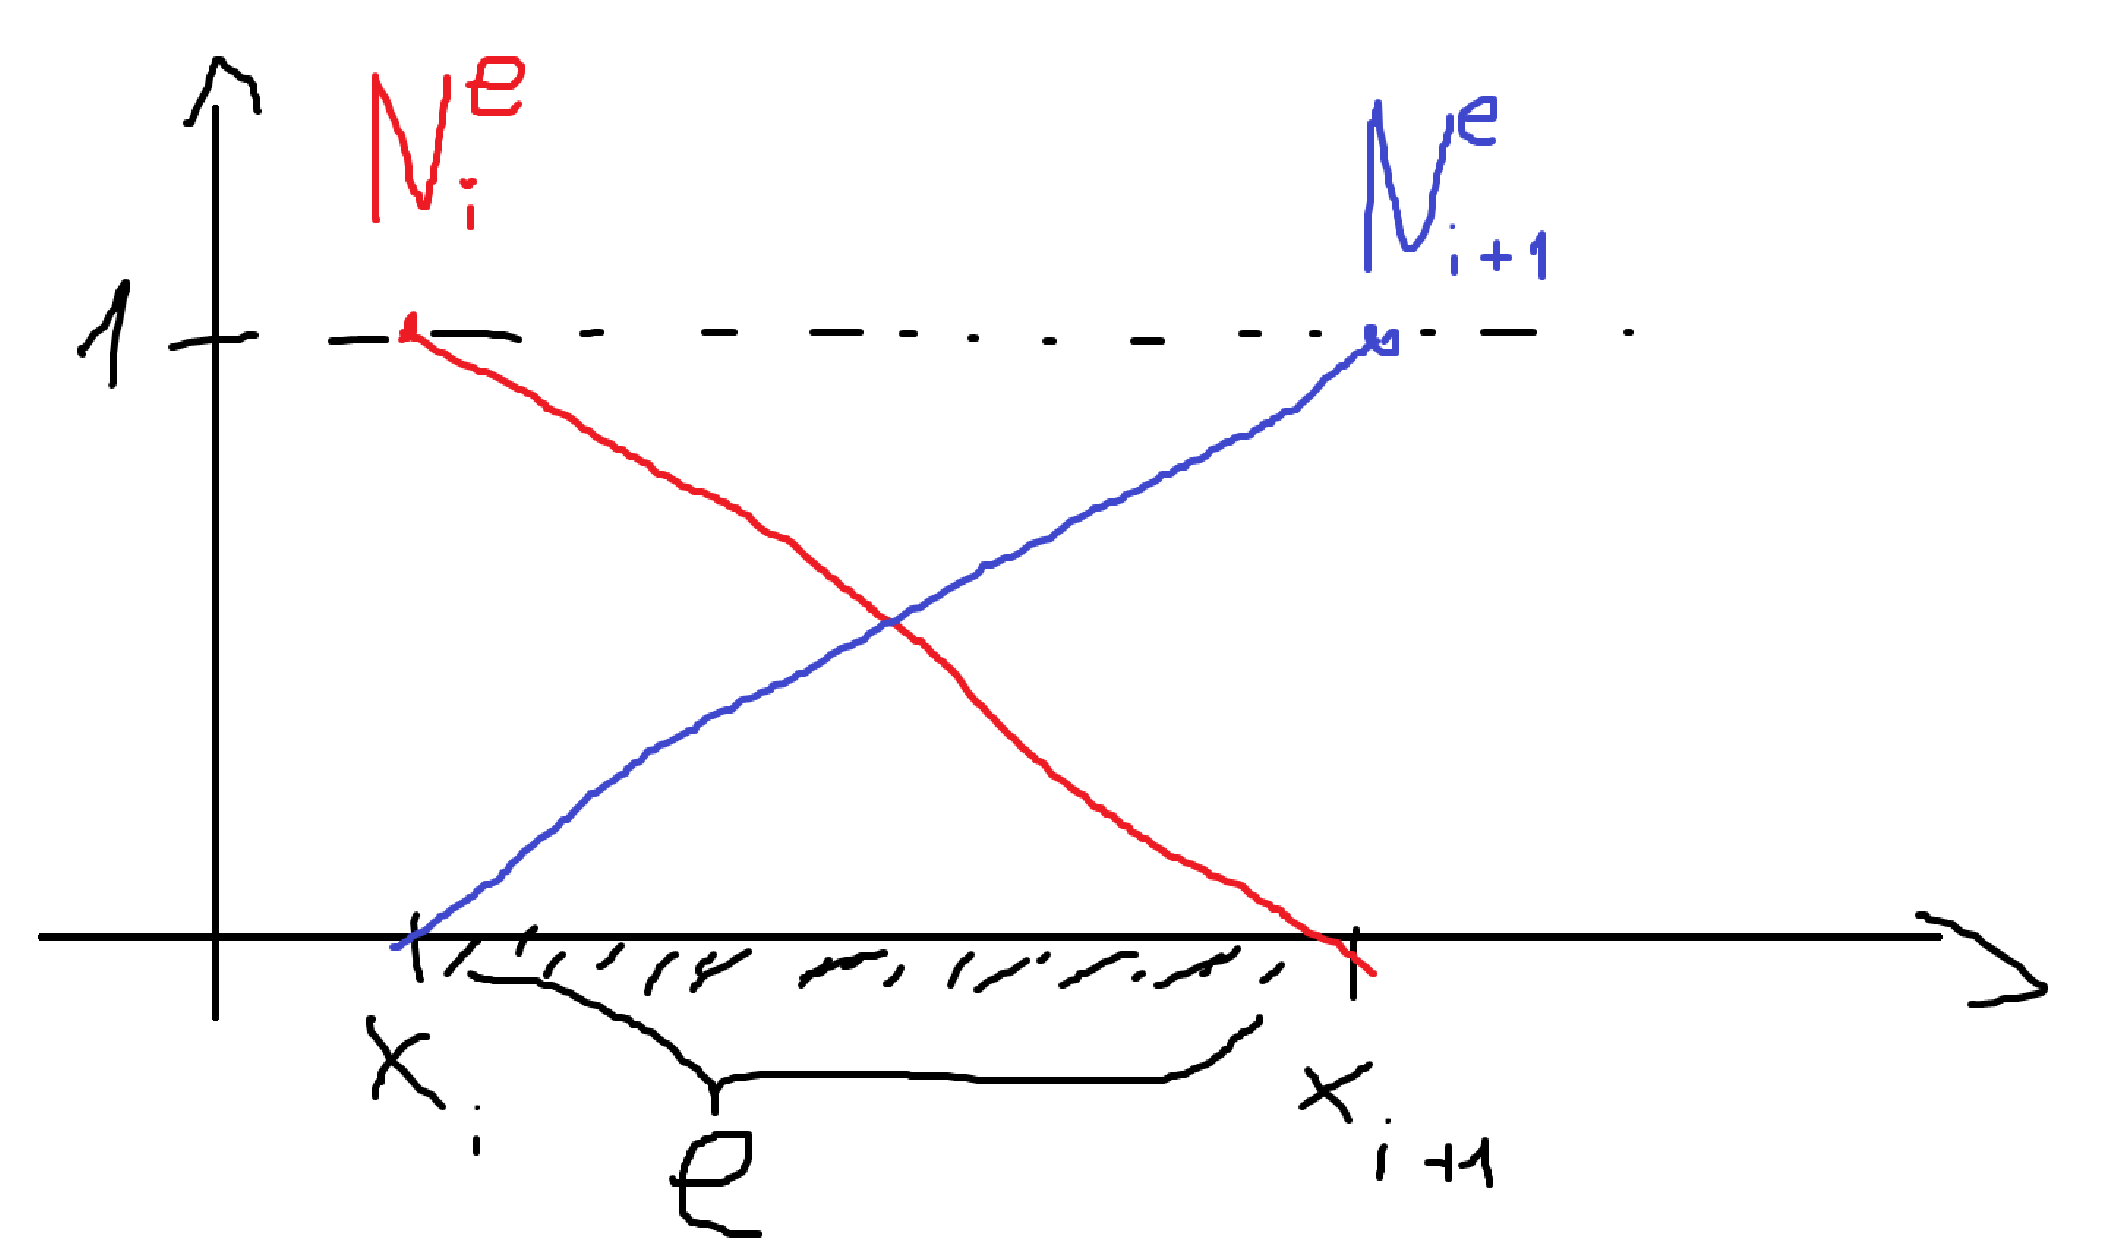
\includegraphics[width=0.4\textwidth]{Images/img_0.png}
  \caption{The piecewise linear basis functions $N^e_i(x)$ and $N^e_{i+1}(x)$ on the 1D element $e$.}
\end{figure}
%

Let's input our finite element approximation $\tilde{y}(x) = \boldsymbol N(x) \boldsymbol{\hat{y}}$ into our volume integral
%
\begin{align}
  \int_{x_1}^{x_n} \frac{ \partial v }{ \partial x } \frac{ \partial \tilde{y} }{ \partial x } \, dx + \int_{x_1}^{x_n} v \, c \, dx                                         & = 0, \\
  \int_{x_1}^{x_n} \left( \frac{ \partial v }{ \partial x } \frac{ \partial \boldsymbol N}{ \partial x } \right) \boldsymbol {\hat{y}} \, dx + \int_{x_1}^{x_n} v \, c \, dx & = 0.
\end{align}

Now, after we make a choice of trial function $v$ in a moment, the only thing unknown in this equation is $\boldsymbol{\hat{y}}$, which we can then solve for.

\subsection{Choosing a \textit{trial function}}
One common choice for the trial function is using the shape functions, as such
%
\begin{equation}
  v(x) \equiv \boldsymbol N(x) \boldsymbol {\delta\hat{y}},
\end{equation}
%
where $\boldsymbol{\delta \hat{y}}$ are random values which crusially aren't functions of $x$. This is called the \textit{Galerkin method}. Inserting this into the volume integral gives us
%
\begin{align}
  \int_{x_1}^{x_n} \frac{ \partial \boldsymbol N }{ \partial x } \boldsymbol {\delta \hat{y}} \frac{ \partial \boldsymbol N}{ \partial x } \boldsymbol {\hat{y}} \, dx + \int_{x_1}^{x_n} \boldsymbol N \boldsymbol {\delta \hat{y}} \, c \, dx      & = 0, \\
  \boldsymbol {\delta \hat{y}}^T\left[\left(  \int_{x_1}^{x_n} \frac{ \partial \boldsymbol N^T }{ \partial x } \frac{ \partial \boldsymbol N}{ \partial x } \, dx \right) \boldsymbol {\hat{y}} + \int_{x_1}^{x_n} \boldsymbol N^T\, c \, dx \right] & = 0.
\end{align}
%
Now we know that the random variables $\boldsymbol{\delta \hat{y}}$ are
non-zero, so therefore we know that the quantity inside the parentheses must be
0:
%
\begin{equation}
  \left(  \int_{x_1}^{x_n} \frac{ \partial \boldsymbol N^T }{ \partial x } \frac{ \partial \boldsymbol N}{ \partial x } \, dx \right) \boldsymbol {\hat{y}} + \int_{x_1}^{x_n} \boldsymbol N^T\, c \, dx = 0.
\end{equation}
%

Since the basis functions $\boldsymbol N$ are just piecewise linear functions, their derivatives must be constant, and thus we can easily evaluate the first term, which becomes a matrix $\boldsymbol K$ times the functions $\boldsymbol{\hat{y}}$. We can also evaluate the second terms, which we define to be the vector $- \mathbf f$. This means that we end up with the linear system $\boldsymbol K \boldsymbol{\hat{y}} = \mathbf f$, where we solve for the unknown $\boldsymbol{\hat{y}}$.
%
\begin{align}
  \underbrace{ \left(  \int_{x_1}^{x_n} \frac{ \partial \boldsymbol N^T }{ \partial x } \frac{ \partial \boldsymbol N}{ \partial x } \, dx \right) \boldsymbol {\hat{y}} }_{ \boldsymbol K \boldsymbol {\hat{y}} } + \underbrace{ \int_{x_1}^{x_n} \boldsymbol N^T\, c \, dx}_{ - \mathbf f } & = 0,             \\
  \boldsymbol K \boldsymbol {\hat{y}} - \mathbf f                                                                                                                                                                                                                                             & = \boldsymbol 0, \\
  \boldsymbol K \boldsymbol {\hat{y}}                                                                                                                                                                                                                                                         & = \mathbf f.
\end{align}
%

\subsection{Computing a solution}
Our linear system has the form
%
\begin{equation}
  \begin{bmatrix}
    K_{11} & \cdots & K_{1n} \\
    \vdots & \ddots & \vdots \\
    K_{n1} & \cdots & K_{nn}
  \end{bmatrix}
  \begin{bmatrix}
    \hat{y}_1 \\
    \vdots    \\
    \hat{y}_n
  \end{bmatrix} = \begin{bmatrix}
    f_1    \\
    \vdots \\
    f_n
  \end{bmatrix}
\end{equation}
%
Enforcing our boundary conditions $y(x_1) = a$ and $y(x_n) = b$ we get
%
\begin{equation}
  \begin{bmatrix}
    1      & \hspace{-8pt} 0            & \hspace{-8pt}\cdots & \hspace{-8pt} 0               & \hspace{-8pt} 0      \\
    0      & \hspace{-8pt} K_{22}       & \hspace{-8pt}\cdots & \hspace{-8pt} K_{2, \, n-1}   & \hspace{-8pt} 0      \\
    \vdots & \hspace{-8pt} \vdots       & \hspace{-8pt}\ddots & \hspace{-8pt} \vdots          & \hspace{-8pt} \vdots \\
    0      & \hspace{-8pt} K_{n-1, \,2} & \hspace{-8pt}\cdots & \hspace{-8pt} K_{n-1, \, n-1} & \hspace{-8pt} 0      \\
    0      & \hspace{-8pt} 0            & \hspace{-8pt}\cdots & \hspace{-8pt} 0               & \hspace{-8pt} 1
  \end{bmatrix}
  \begin{bmatrix}
    \hat{y}_1     \\
    \hat{y}_2     \\
    \vdots        \\
    \hat{y}_{n-1} \\
    \hat{y}_n
  \end{bmatrix} = \begin{bmatrix}
    a                                     \\
    f_2 - K_{21} a - K_{2n} b             \\
    \vdots                                \\
    f_{n-1} - K_{n-1, 1} a - K_{n-1, n} b \\
    b
  \end{bmatrix},
\end{equation}
%
We call this the modified linear system
%
\begin{equation}
  \boldsymbol {K'} \boldsymbol {\hat{y}} = \mathbf{f'},
\end{equation}
%
and this can be solved.

\section{Generalization to 2D}
The equivalent problem in 2D can be formulated as such:
Given a domain $\Omega \in \mathbb{R}^2$ with boundary $\partial\Omega$, we want to find the function $u(\boldsymbol p) : \mathbb{R}^2 \to \mathbb{R} ; \ \boldsymbol p \in \Omega$, such that
%
\begin{align}
  \frac{ \partial^{2} u(\boldsymbol p) }{ \partial x^{2} } + \frac{ \partial^{2} u(\boldsymbol p) }{ \partial y^{2} }  = c(\boldsymbol p) & ; \quad c(\boldsymbol p): \mathbb{R}^2 \to \mathbb{R} \\
  u(\boldsymbol p) = a(\boldsymbol p)                                                                                                     & ; \quad \forall \boldsymbol p \in \partial \Omega.
\end{align}
%
\begin{figure}[H]
  \centering
  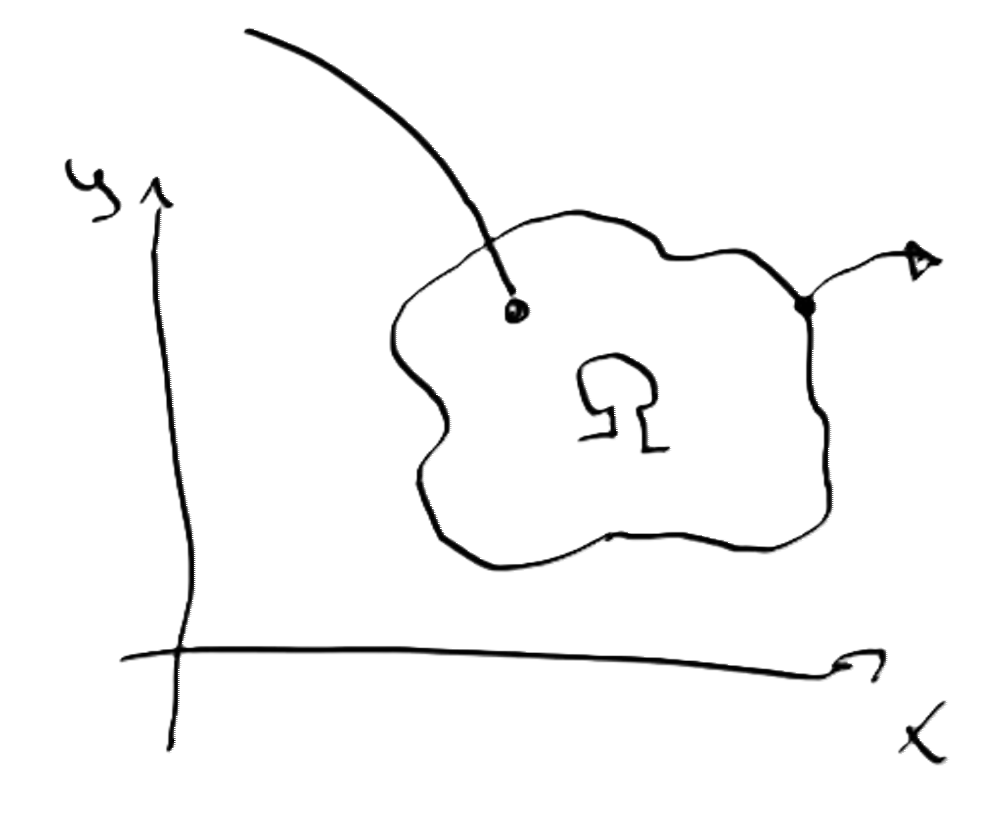
\includegraphics[width=0.2\textwidth]{Images/img_1.png}
  \caption{A 2D domain $\Omega$ with boundary $\partial \Omega$ .}
\end{figure}
%

After acquiring a mesh of our domain by whatever means, we observe that the elements on the boundary become lines, and the elements on the inside become triangles. Each vertex in the mesh is associated with a set of coordinates $(x_i, \ y_i)$ and an unknown function value $u_i$, which we want to solve for.
%
\begin{figure}[H]
  \centering
  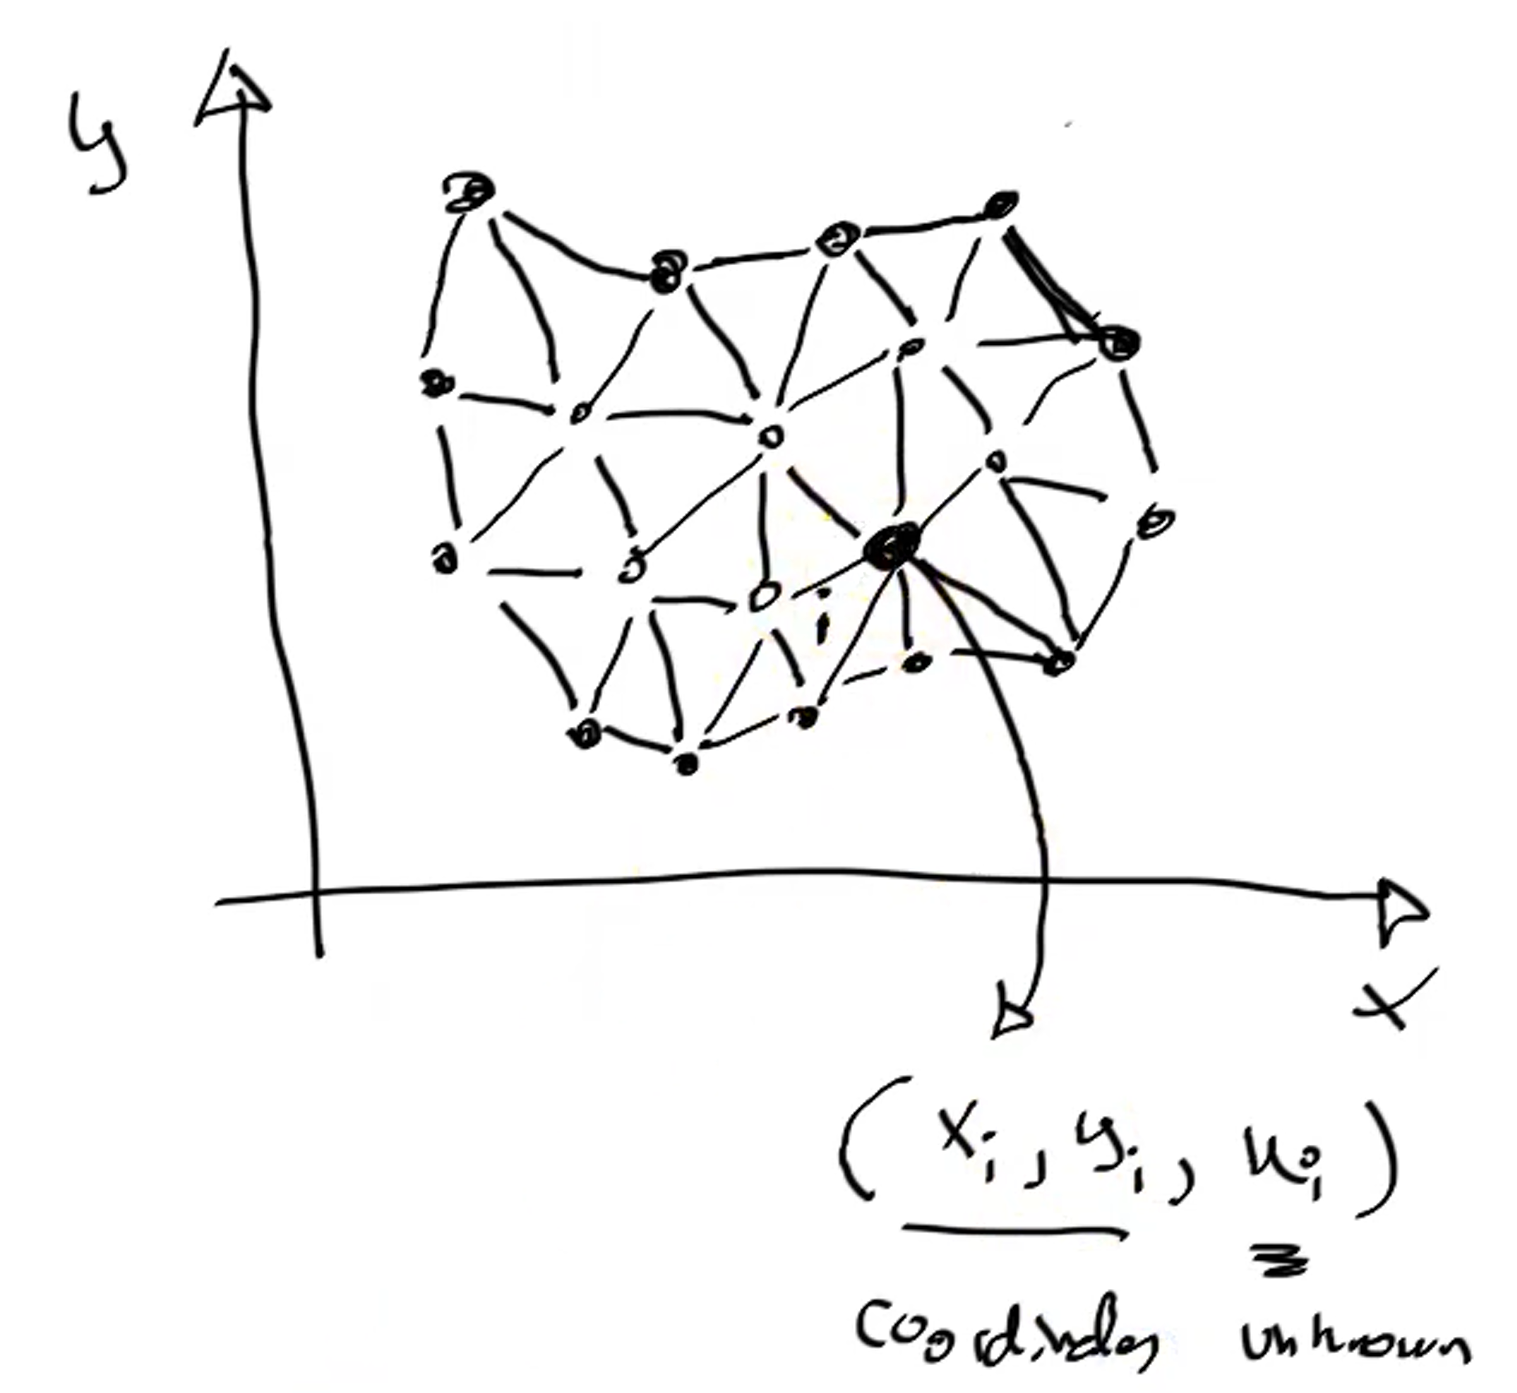
\includegraphics[width=0.3\textwidth]{Images/img_2.png}
  \caption{A mesh of our domain.}
\end{figure}
%

\subsection{The linear shape functions in 2D}
The $e$'th element in our mesh has three vertices $(i,j,k)$ and the finite element approximation of $u(\boldsymbol p)$ in this 2D scenario takes the form:
%
\begin{equation}
  u^e(\boldsymbol p) \approx \tilde{u}^e(\boldsymbol p) = \begin{bmatrix}
    N_i^e(\boldsymbol p) & N_j^e(\boldsymbol p) & N_k^e(\boldsymbol p)
  \end{bmatrix} \begin{bmatrix}
    \hat{u}_i^e(\boldsymbol p) \\ \hat{u}_j^e(\boldsymbol p) \\ \hat{u}_k^e(\boldsymbol p)
  \end{bmatrix}.
\end{equation}
%
\begin{figure}[H]
  \centering
  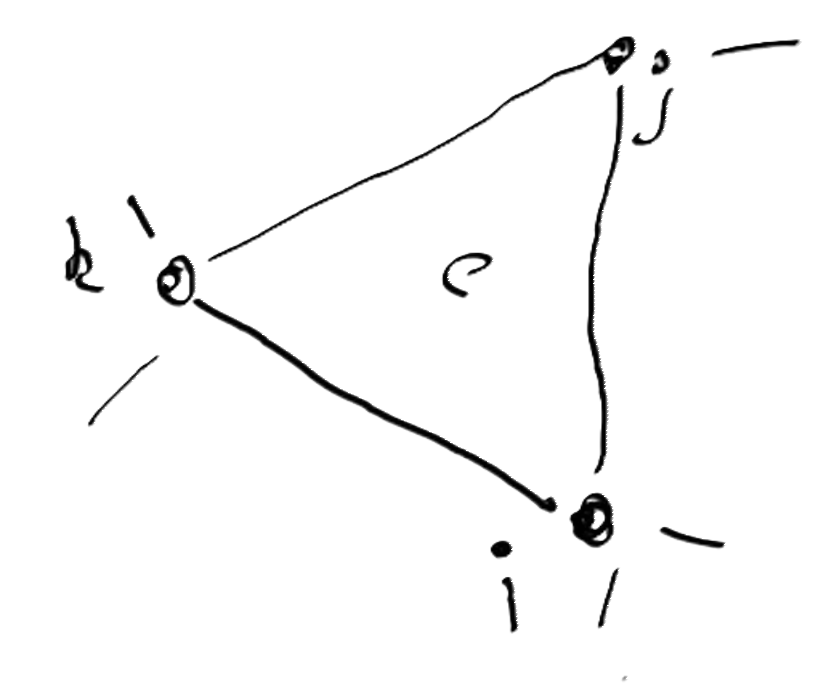
\includegraphics[width=0.2\textwidth]{Images/img_3.png}
  \caption{An element $e$ of our mesh with vertices $(i,j,k)$}
\end{figure}
%

Like in 1D, the shape functions are defined to be 1 in their respective node, and $0$ in the other nodes, with linear slope between the nodes.
\begin{figure}[H]
  \centering
  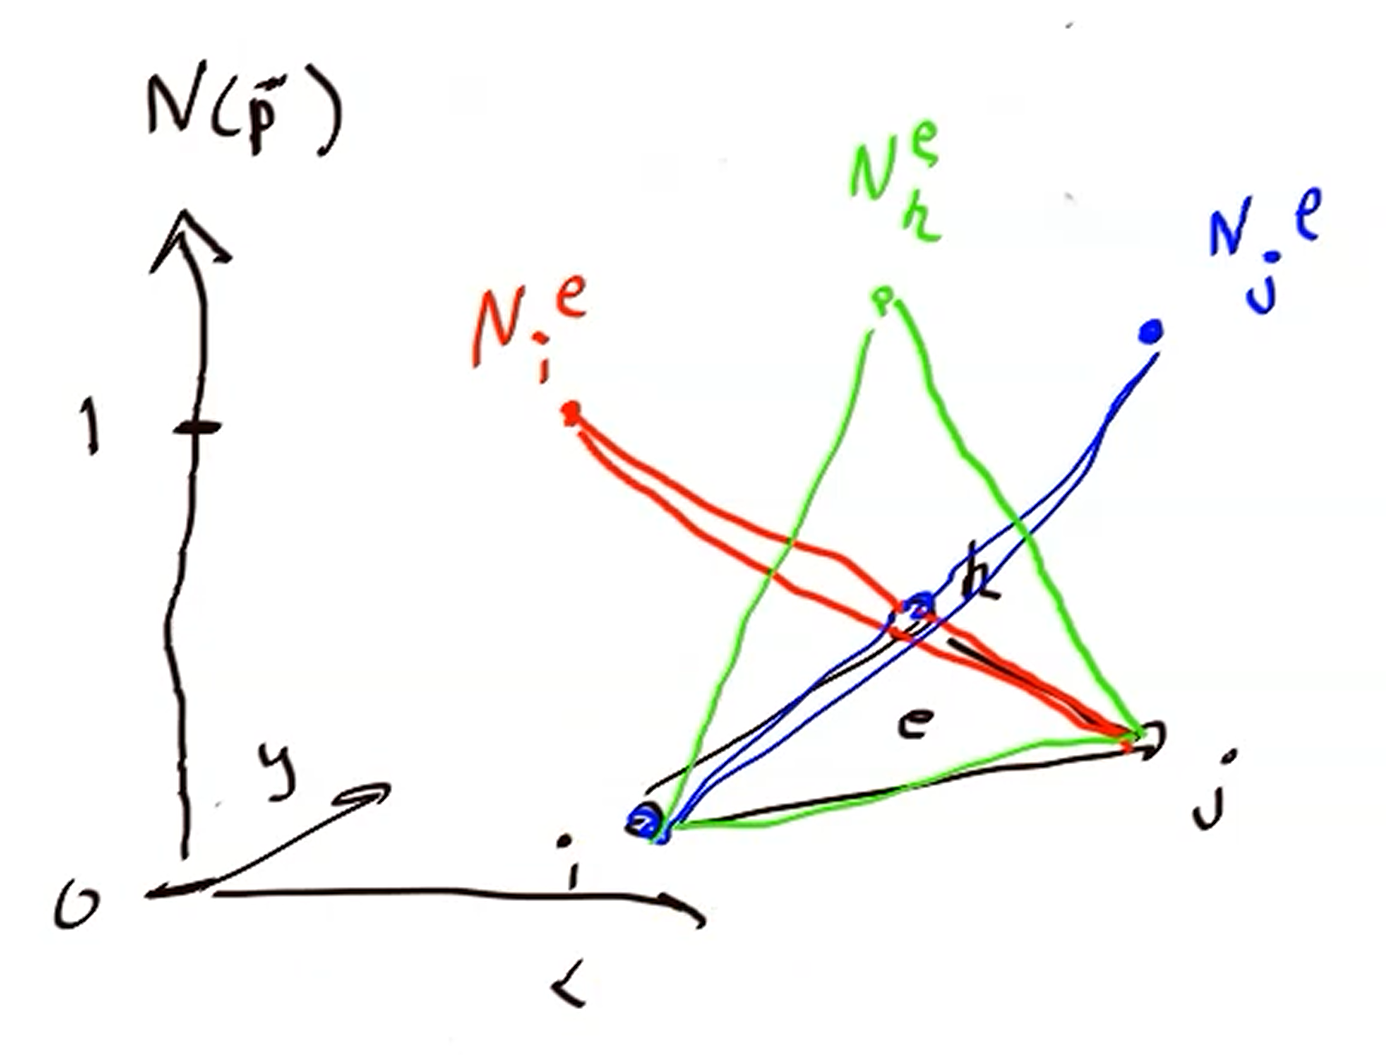
\includegraphics[width=0.3\textwidth]{Images/img_4.png}
  \caption{The shape functions $\boldsymbol N^e$ of an element $e$.}
\end{figure}
%

Given a point $\boldsymbol p$ in our element, we can convince ourselves, that the full area of the element is going to be the sum of the 3 partitions of the triangle defined by the point as in figure \ref{fig:area_partitions}
%
\begin{equation}
  A_{ijk} = A_{jk \boldsymbol p} + A_{ki \boldsymbol p} + A_{ij \boldsymbol p}.
\end{equation}
%
\begin{figure}[H]
  \centering
  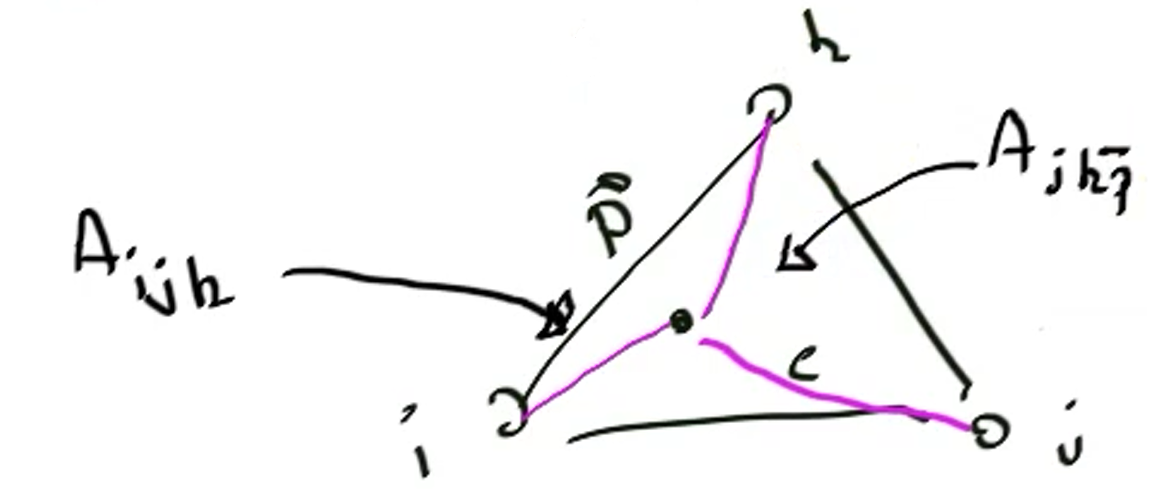
\includegraphics[width=0.3\textwidth]{Images/img_5.png}
  \caption{The relevant areas formed by a point $\boldsymbol p$ somewhere on the element and the vertices of the element. \label{fig:area_partitions}}
\end{figure}
%

Defining $\boldsymbol N^e = \big(N_i^e, \ N_j^e, \ N_k^e\big)^T,$ with
%
\begin{equation}
  N_i^e = \frac{A_{jk \boldsymbol p}}{A_{ijk}}, \qquad\quad N_j^e = \frac{A_{ki \boldsymbol p}}{A_{ijk}}, \qquad\quad N_k^e = \frac{A_{ij \boldsymbol p}}{A_{ijk}},
\end{equation}
%
we get
%
\begin{equation}
  1 = N_i^e + N_j^e + N_k^e,
\end{equation}
%
which also ensures that the condition for \textit{partition of units}  is satisfied.

Now, using vectors we can easily compute the areas using cross products, since this calculates the area of the parallelogram spanned by the two vectors
%
\begin{equation}
  A_{ijk} = \frac{1}{2} (\boldsymbol p_j - \boldsymbol p_i) \times (\boldsymbol p_k - \boldsymbol p_i).
\end{equation}
%
Using this result, we can obtain
%
\begin{align}
  N_i^e & = \frac{(\boldsymbol p_k - \boldsymbol p_j) \times (\boldsymbol p - \boldsymbol p_j)}{2 A_{ijk}}, \\
  N_j^e & = \frac{(\boldsymbol p_i - \boldsymbol p_k) \times (\boldsymbol p - \boldsymbol p_k)}{2 A_{ijk}}, \\
  N_k^e & = \frac{(\boldsymbol p_j - \boldsymbol p_i) \times (\boldsymbol p - \boldsymbol p_i)}{2 A_{ijk}},
\end{align}
%
the first of which has the derivatives
%
\begin{equation}
  \frac{ \partial N_i^e }{ \partial x } = \frac{(\boldsymbol p_k - \boldsymbol p_j)}{2 A_{ijk}} \times \frac{ \partial \boldsymbol p }{ \partial x }, \qquad \frac{ \partial N_i^e }{ \partial y } = \frac{(\boldsymbol p_k - \boldsymbol p_j)}{2 A_{ijk}} \times \frac{ \partial \boldsymbol p }{ \partial y }.
\end{equation}
%
Now, since $\boldsymbol p = (x, y)^T$ we have $\partial \boldsymbol p/\partial x = (1, 0)^T = \boldsymbol{\hat{\imath}}$ and $\partial \boldsymbol p/\partial y = (0, 1)^T = \boldsymbol{\hat{\jmath}}$. Taking the crossproduct between any 2d vector $\boldsymbol a$ and the unit vectors $\boldsymbol{\hat{\imath}}$ or $\boldsymbol{\hat{\jmath}}$ yields
%
\begin{equation}
  \boldsymbol a \times \boldsymbol{\hat{\imath}} = -a_y, \qquad \text{and}\qquad \boldsymbol a \times \boldsymbol{\hat{\jmath}} = a_x,
\end{equation}
%
which means that
%
\begin{align}
  \frac{ \partial N_i^e }{ \partial x } & = -\frac{\big[\boldsymbol p_k - \boldsymbol p_j\big]_y}{2 A_{ijk}}, \qquad \frac{ \partial N_i^e }{ \partial y } = \frac{\big[\boldsymbol p_k - \boldsymbol p_j\big]_x}{2 A_{ijk}}, \\
  \frac{ \partial N_j^e }{ \partial x } & = -\frac{\big[\boldsymbol p_i - \boldsymbol p_k\big]_y}{2 A_{ijk}}, \qquad \frac{ \partial N_j^e }{ \partial y } = \frac{\big[\boldsymbol p_i - \boldsymbol p_k\big]_x}{2 A_{ijk}}, \\
  \frac{ \partial N_k^e }{ \partial x } & = -\frac{\big[\boldsymbol p_j - \boldsymbol p_i\big]_y}{2 A_{ijk}}, \qquad \frac{ \partial N_k^e }{ \partial y } = \frac{\big[\boldsymbol p_j - \boldsymbol p_i\big]_x}{2 A_{ijk}}.
\end{align}
%
Defining $(\boldsymbol p_j - \boldsymbol p_i) = \boldsymbol p_{ij}$, we obtain a more compact form of the derivatives
%
\begin{equation}
  \frac{ \partial N_i^e }{ \partial \boldsymbol p } = \frac{\hat{\boldsymbol p}_{jk}}{2 A_{ijk}}, \qquad \frac{ \partial N_j^e }{ \partial \boldsymbol p } = \frac{\hat{\boldsymbol p}_{ki}}{2 A_{ijk}}, \qquad \frac{ \partial N_k^e }{ \partial \boldsymbol p } = \frac{\hat{\boldsymbol p}_{ij}}{2 A_{ijk}},
\end{equation}
%
where we make use of the hat operator $\boldsymbol {\hat a} = (-a_y, a_x)^T$. Note that these are constant wrt. $x$ and $y$, since they only depend on the vertices of the mesh element, which is static.

\subsection{Applying the FEM on a 2D problem}
Looking at a specific element of our mesh with domain $\Omega^e$, which has one side on the boundary of our domain $\Gamma^e \in \partial\Omega$, we can formulate the volume integral over the element as such
%
\begin{multline}
  \int_{\Omega^e} v^e(\boldsymbol p) \left( \frac{ \partial^{2} u }{ \partial x^{2} } + \frac{ \partial^{2} u }{ \partial y^{2} } - c(\boldsymbol  p) \right) \, d\Omega\\
  + \int_{\Gamma^e} w^e(\boldsymbol p) (u(\boldsymbol  p) - a(\boldsymbol p)) \, d\Gamma = 0.
\end{multline}
%
\begin{figure}[H]
  \centering
  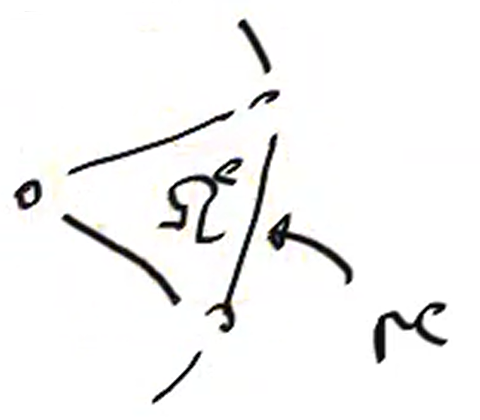
\includegraphics[width=0.2\textwidth]{Images/img_6.png}
  \caption{A specific element of our mesh with domain $\Omega^e$ which has one side on the boundary of our domain $\Gamma^e$.\label{fig:ele_on_bound}}
\end{figure}
%

Now, it should be said that $\Gamma^e$ here, is not the whole boundary of the element $e$, but only the part of it, that also happens to coincide with the boundary of our mesh domain $\partial\Omega$ (see figure \ref{fig:ele_on_bound}).

Looking at the first term, we get
%
\begin{equation}
  \int_{\Omega^e} \frac{ \partial v^e }{ \partial x }  \frac{ \partial u }{ \partial x } \, d\Omega + \int_{\Omega^e} \frac{ \partial v^e }{ \partial y }  \frac{ \partial u }{ \partial y } \, d\Omega - \int_{\Omega^e} v^e c \, d\Omega = 0,
\end{equation}
%
where we've used integration by parts and the fact that our trial function is 0 on the boundaries (see the 1D case for clarification).
Now using the FEM approximation $u^e \approx \tilde{u}^e = \boldsymbol N^e \boldsymbol{\hat{u}}^e$ and the \textit{Galerkin assumption}  $v^e = \boldsymbol N^e \boldsymbol{\delta \hat{v}}$, we arrive at (using the same steps as for the 1D case)
%
\begin{equation}
  \left(  \int_{\Omega^e} \frac{ \partial {{\boldsymbol N}^e}^T }{ \partial x } \frac{ \partial \boldsymbol N^e}{ \partial x } + \frac{ \partial {{\boldsymbol N}^e}^T }{ \partial y } \frac{ \partial \boldsymbol N^e}{ \partial y } \, d\Omega\right) \boldsymbol {\hat{u}}^e + \int_{\Omega^e} {{\boldsymbol N}^e}^T\, c \, d\Omega = 0.
\end{equation}
%
As we saw above, the derivatives of our shape functions $\boldsymbol N^e$ are constant wrt. $x$ and $y$ and thus, this becomes
%
\begin{equation}
  \underbrace{ A_{ijk} \left[  \frac{ \partial {{\boldsymbol N}^e}^T }{ \partial x } \frac{ \partial \boldsymbol N^e}{ \partial x } + \frac{ \partial {{\boldsymbol N}^e}^T }{ \partial y } \frac{ \partial \boldsymbol N^e}{ \partial y }\right] }_{ \boldsymbol K^e } \boldsymbol{\hat{u}}^e - \mathbf f^e = 0.
\end{equation}
%

\section{Discussion of grid characteristics}
The choice of grid spacing is important in the FEM method. If we choose a grid spacing that is too large, we might miss important features of the solution, and if we choose a grid spacing that is too small, we might end up with a system that is too computationally expensive to solve.

The finite element method is powerful in the sense that it allows us to have a non-uniform grid, but we have to be careful with this. The reason is, that, in our formalism, the shape functions $\boldsymbol N^e$ are piecewise linear functions, making our interpolated field values $\boldsymbol u(\boldsymbol x)$ linear approximations, which are dependent on the geometry of the elements. Therefore, if we have a non-uniform grid, the quality and accuracy of our solution might be poorer in some regions than others, and this might affect the solution.

We might also concieve of a scenario where the mesh is constructed in a way such that it's regular along two axes, but not in any direction, like in figure \ref{fig:ani_grid}. This might lead to the error of our solution different along different directions, which is not ideal, especially if we're interested in modelling anisotropic materials or objects with complex geometries, such as structural elements of vehicles, etc.
%
\begin{figure}[H]
  \centering
  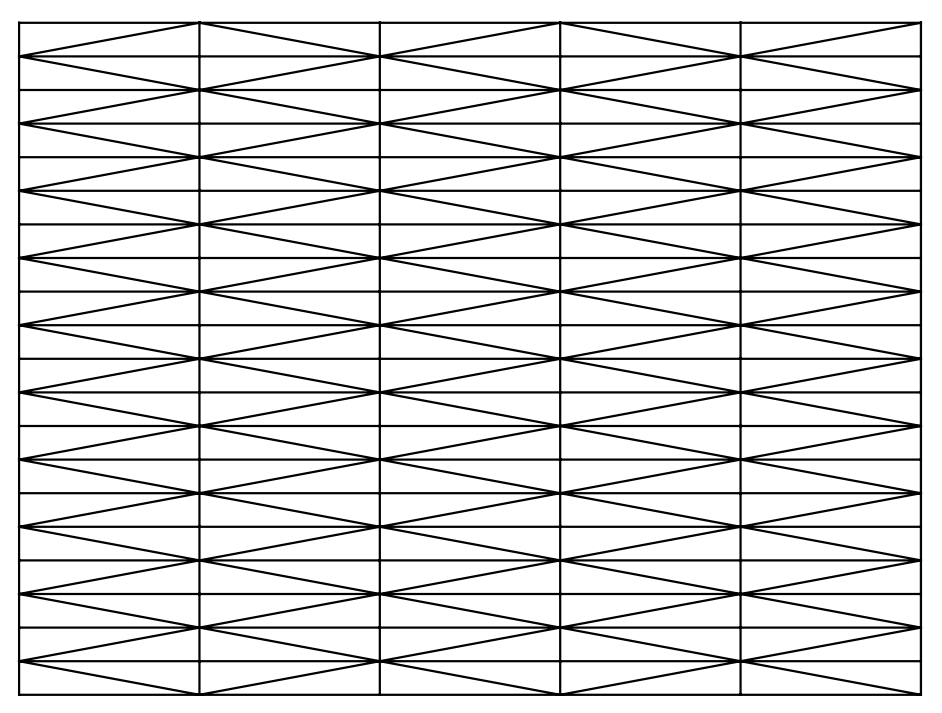
\includegraphics[width=0.3\textwidth]{Images/ani_grid.png}
  \caption{Example of a grid that is regular along two axes, but not in any direction.\label{fig:ani_grid}}
\end{figure}
%

The material from week 3 is also very relevant here, as the quality measures are directly related to the regularity of the elements, and thus the uniformity of the mesh. Since the shape functions are linear approximations, which are dependent on the geometries of the mesh elements, the error of our result is directly related to the quality of the elements and thus the uniformity of our grid.

\section{Experiments}
\subsection*{Experiment 1: Performance for different grid partitions}
In this experiment, we want to investigate the performance of our FEM solver for different grid partitions. We want to see how the error and runtime of our solver changes as we increase the number of grid partitions.

We start by calculating the solution for grid partitions $I = 100$, which we will take to be the reference solution. We then calculate the solution for grid partitions $I \in (7, 96)$ and plot the error and runtime as a function of the number of grid partitions. We expect to see a decrease in error and an increase in runtime as we increase the number of grid partitions, and that's exactly what we see in figure \ref{fig:w4exp1}.

\graphicspath{{Images/Week4/exp1/}}
\begin{figure}[t]
  \centering
  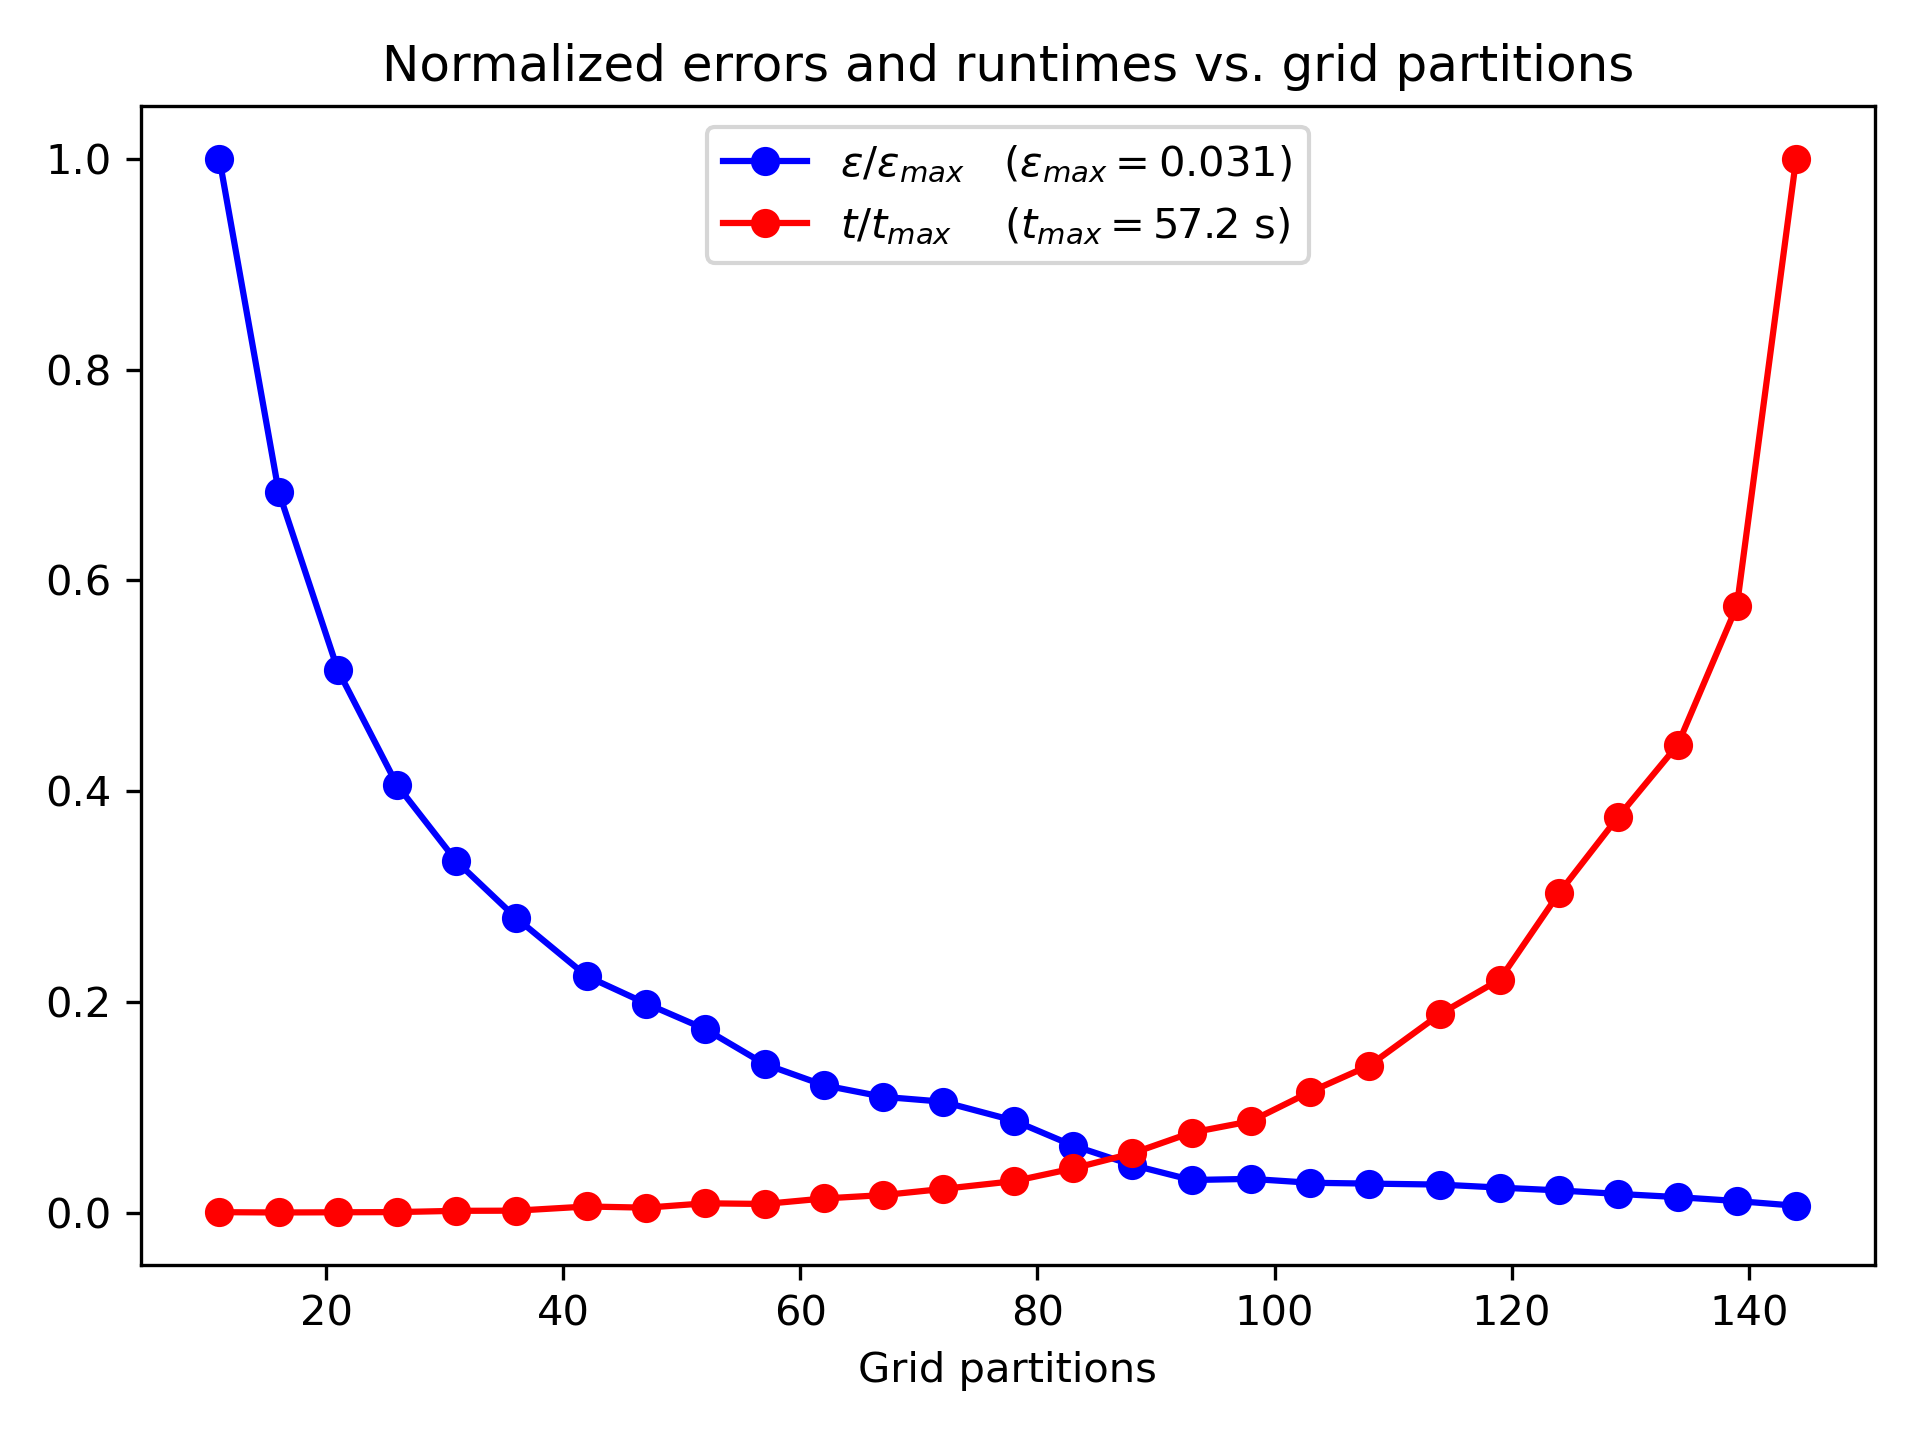
\includegraphics[width = 0.3\textwidth]{Normalized_errors_runtimes_vs_grid_partitions.png}
  \caption{The errors and runtimes of our solution for different grid partitions.\label{fig:w4exp1}}
\end{figure}

\subsection{Experiment 2: Stretching the domain}
In this experiment, we want to see how the solution behaves when the domain is stretched along one direction. We choose the boundary conditions to be two linear functions with opposite slope, lying at the left and right boundaries $x_\mathrm{left}$ and $x_\mathrm{right}$. We then calculate the solution for the domains $\left\lVert x_\mathrm{right} - x_\mathrm{left} \right\rVert  = 1, 2, 4$ and plot the solution.

Our physical intuition dictates, that we expect the non-zero parts of the solution to decay at an exponential rate with constant exponent, and thus, the wider domain will have a large flat zero-valued region in the middle. This is exactly what we see in figures \ref{fig:w4exp2_0}, \ref{fig:w4exp2_1} and \ref{fig:w4exp2_2}.

\graphicspath{{Images/Week4/exp2/}}
\begin{figure}[t]
  \centering
  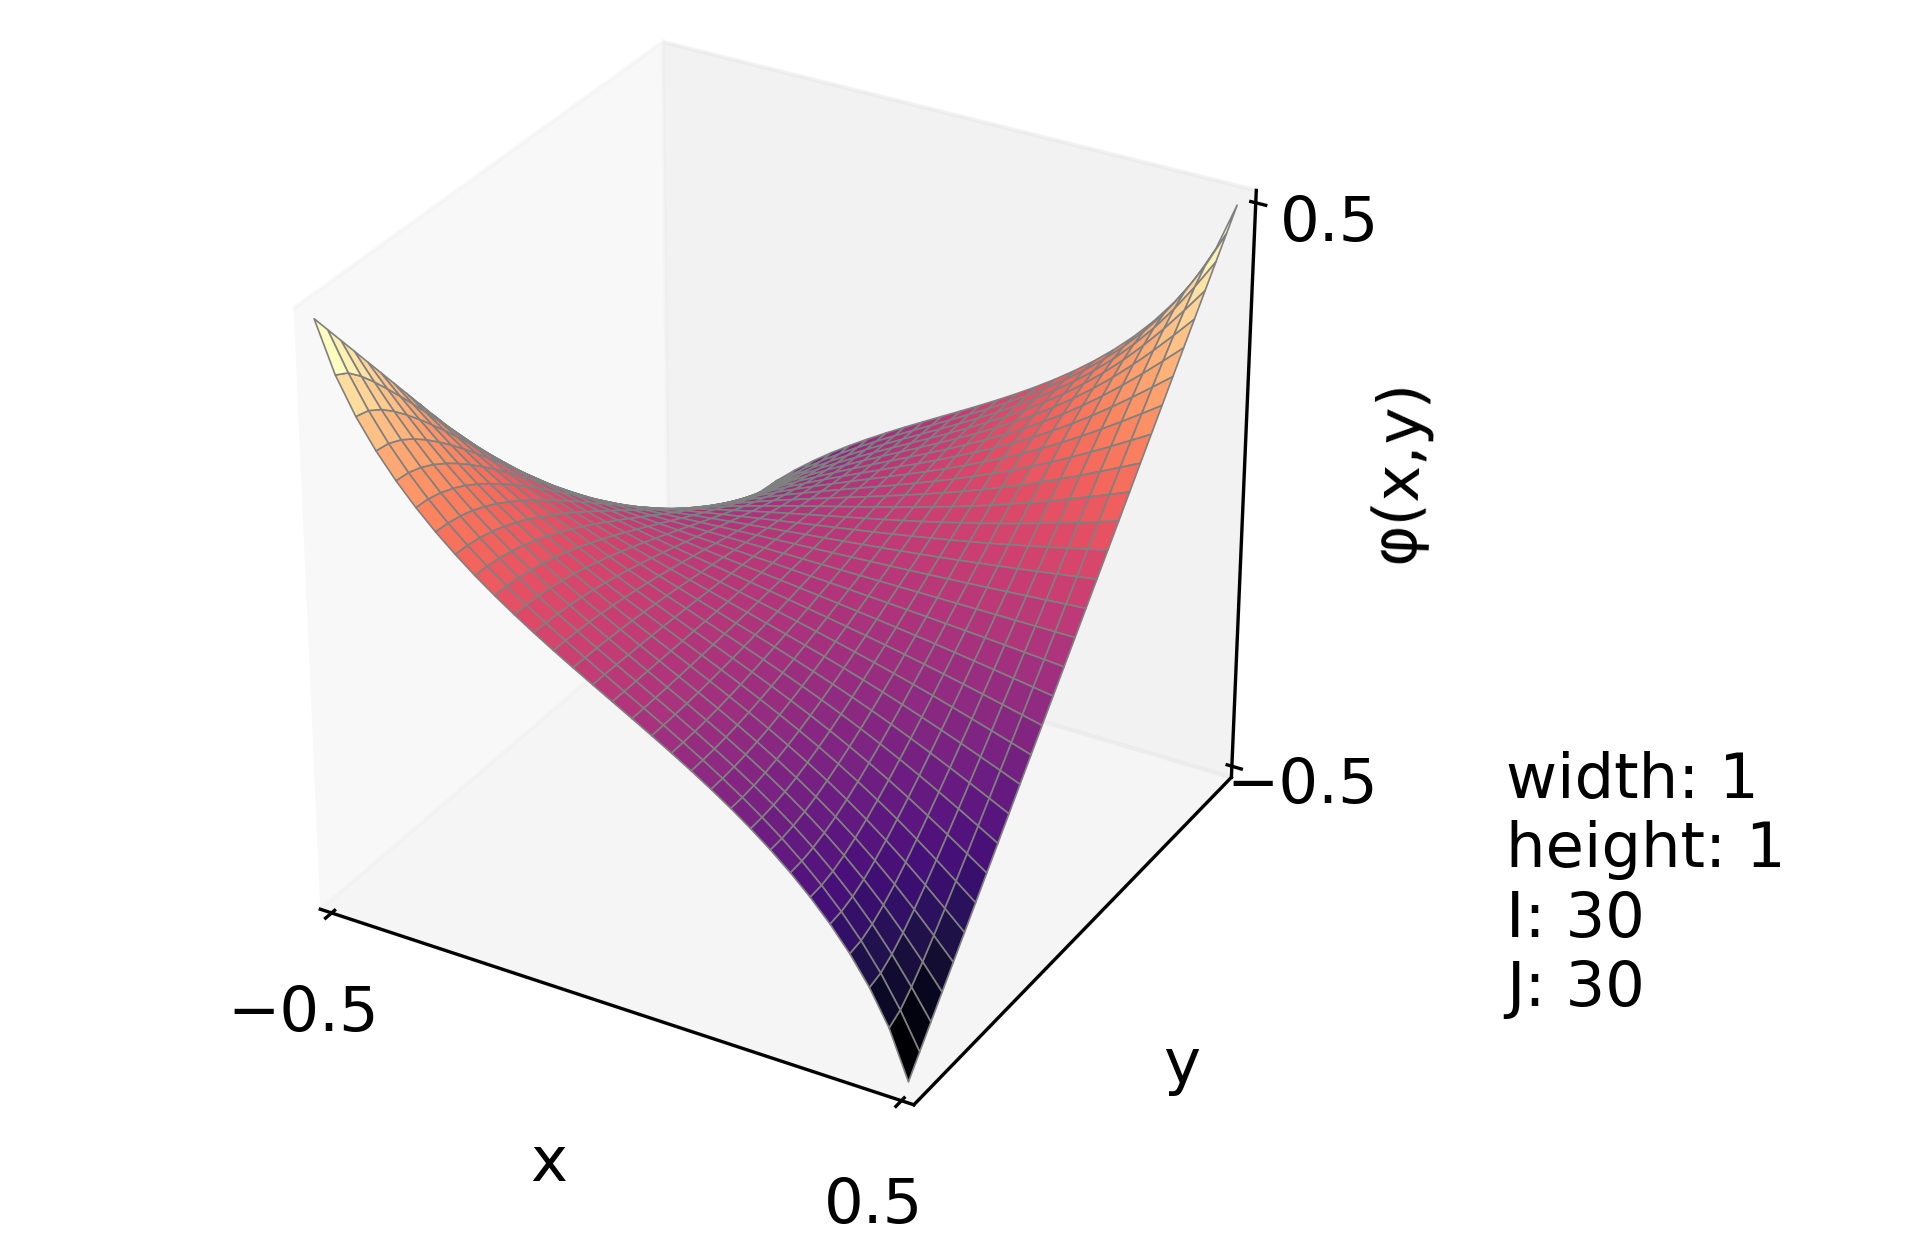
\includegraphics[width = 0.4\textwidth]{widths_0.png}
  \caption{Solution for domain of width 1.\label{fig:w4exp2_0}}
\end{figure}
\begin{figure}[t]
  \centering
  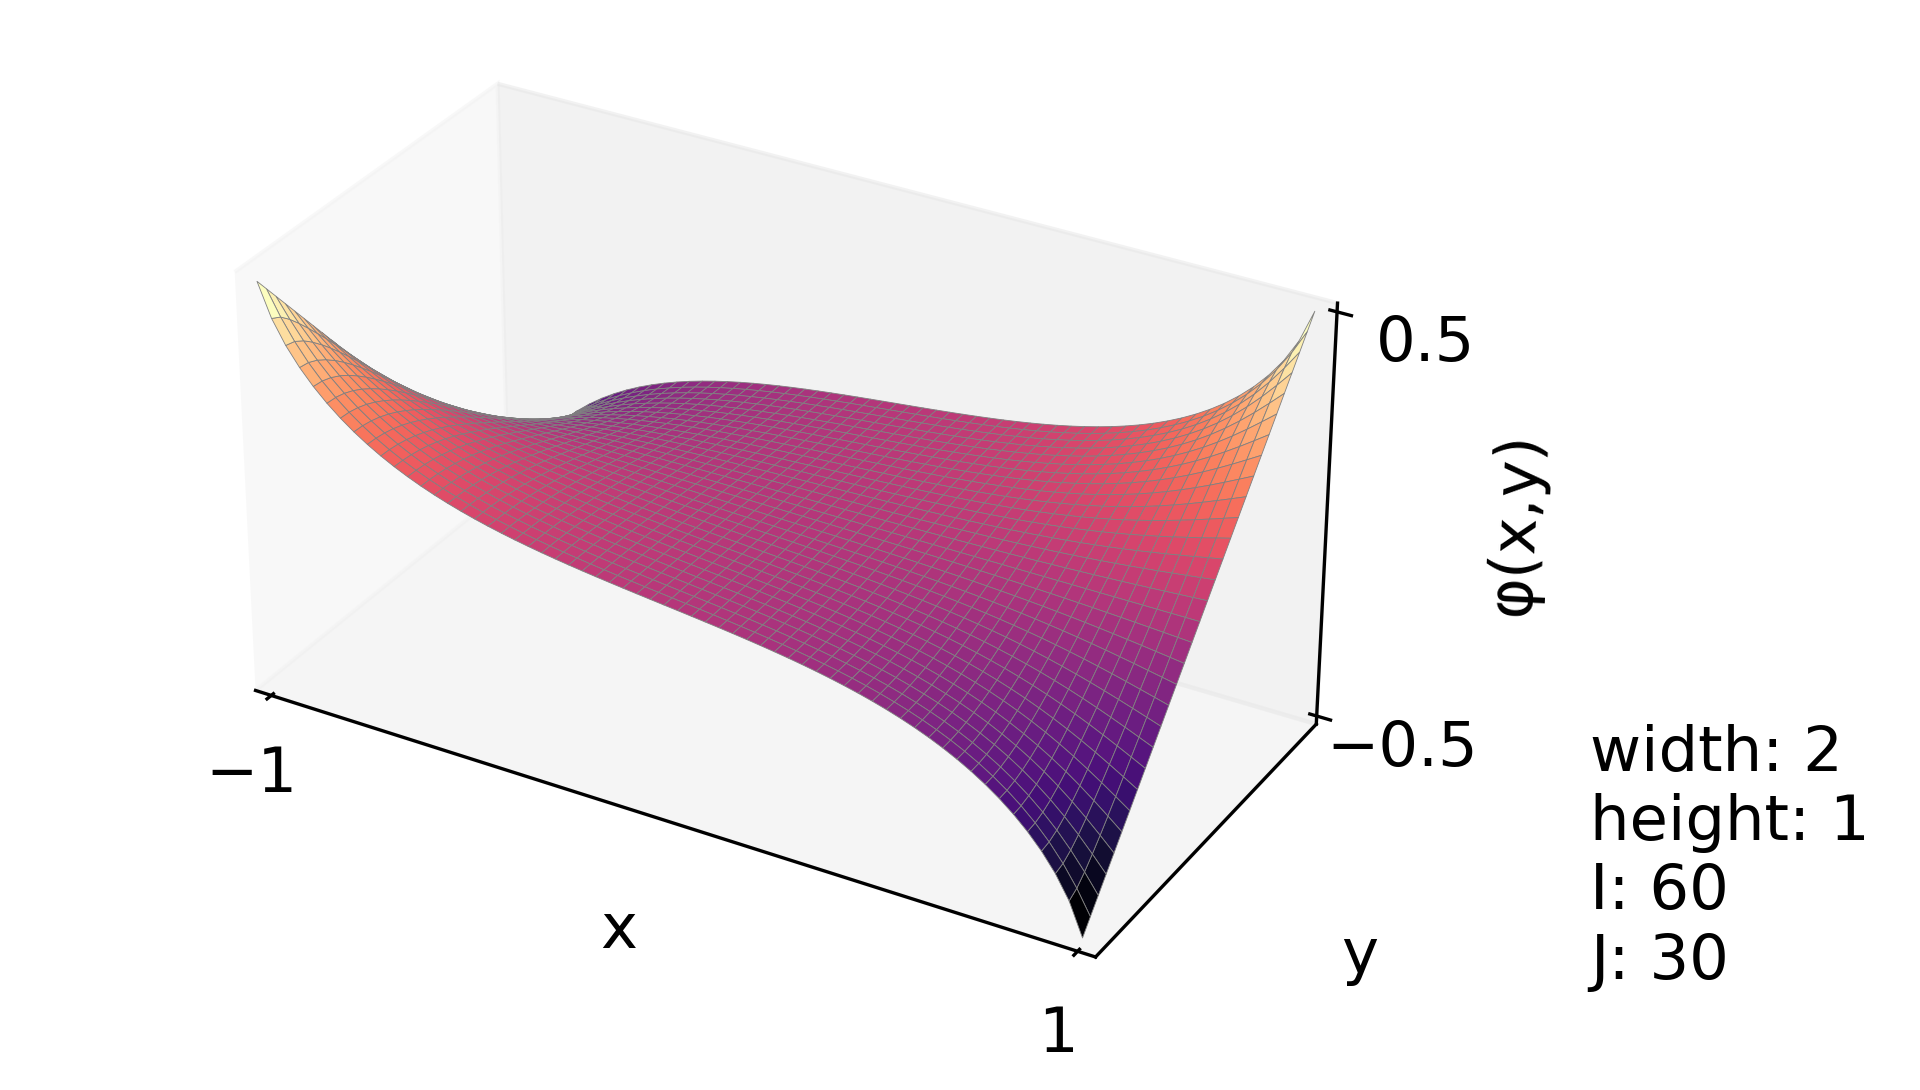
\includegraphics[width = 0.4\textwidth]{widths_1.png}
  \caption{Solution for domain of width 2.\label{fig:w4exp2_1}}
\end{figure}
\begin{figure}[t]
  \centering
  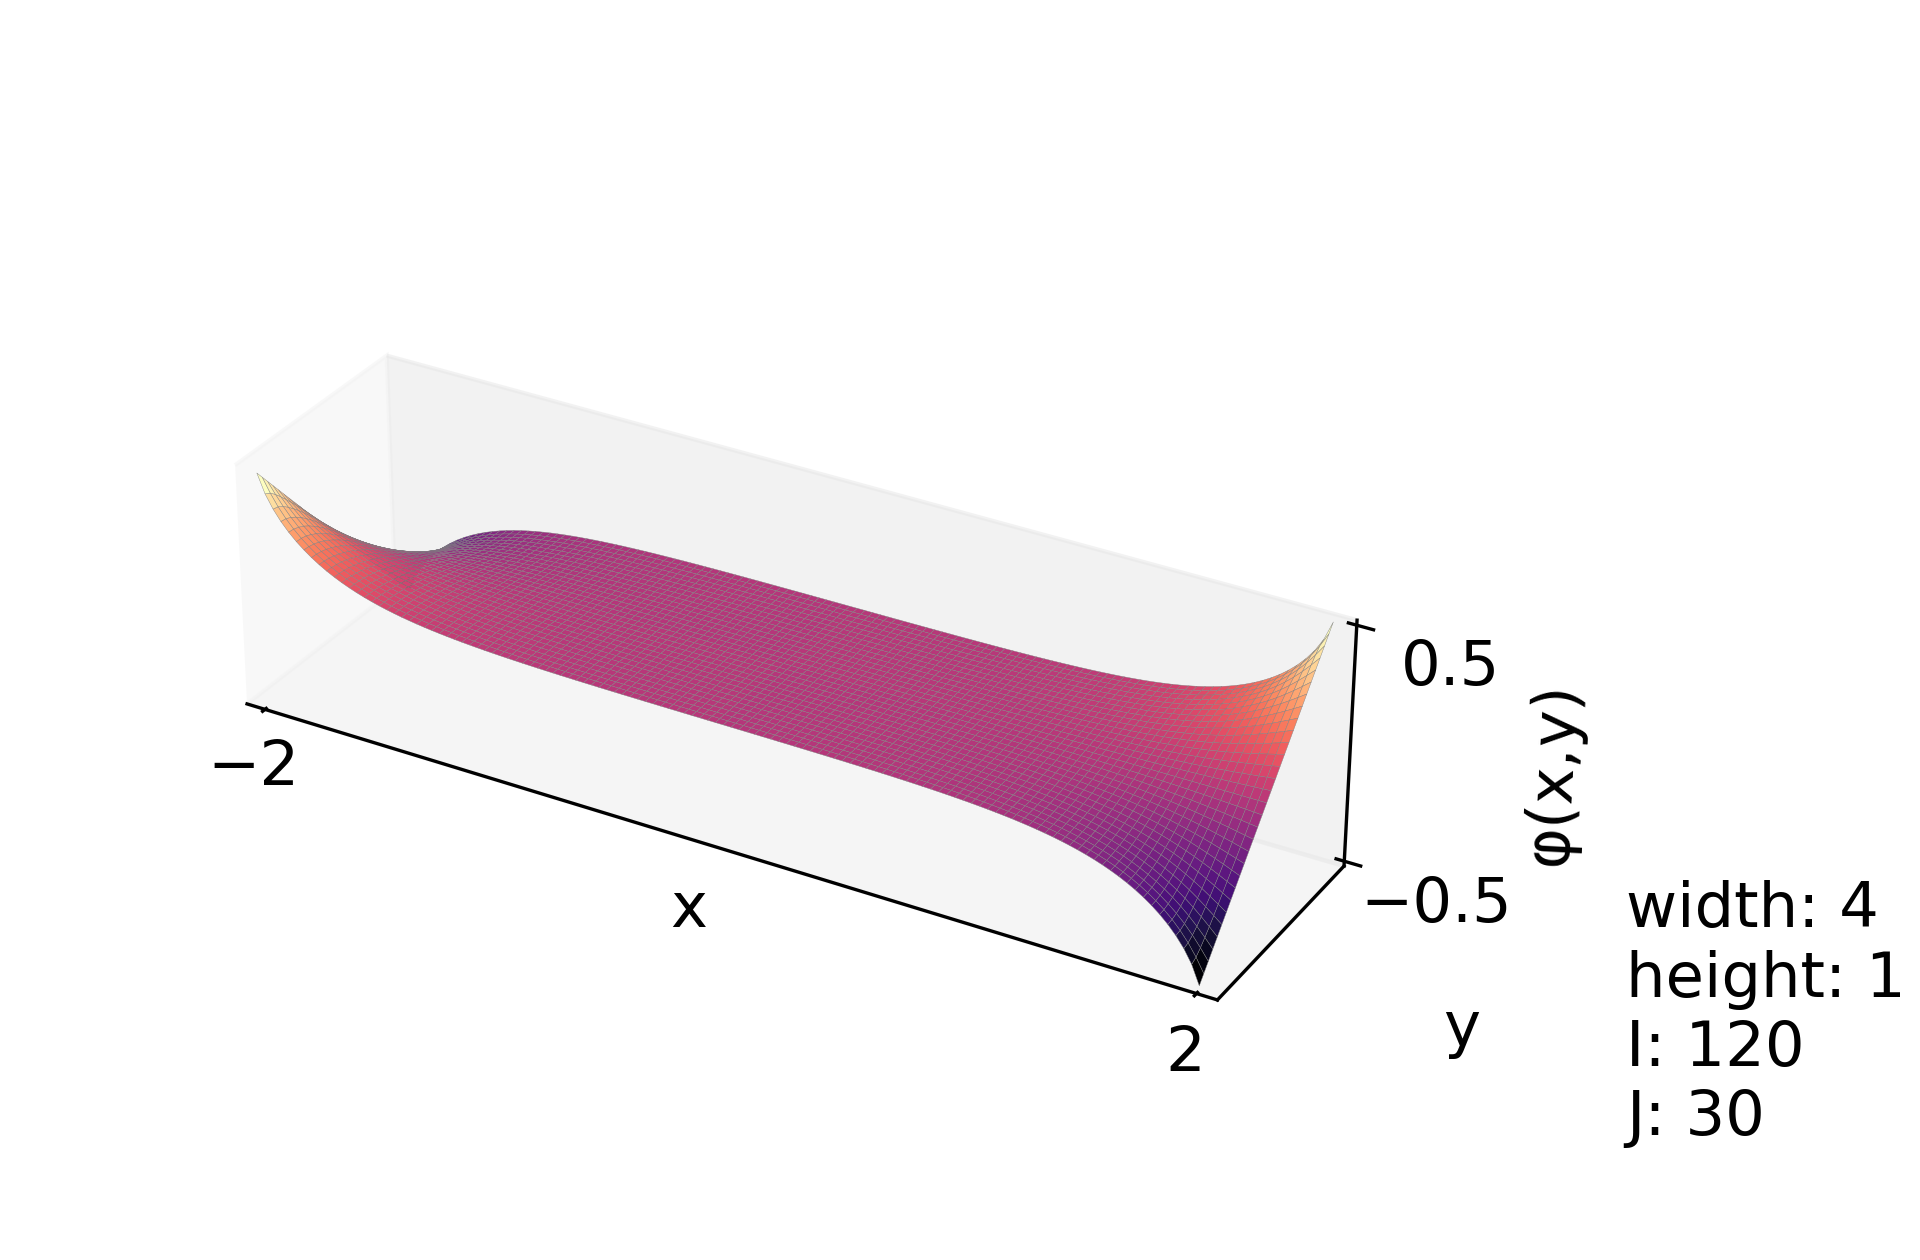
\includegraphics[width = 0.4\textwidth]{widths_2.png}
  \caption{Solution for domain of width 4.\label{fig:w4exp2_2}}
\end{figure}



\vspace{12pt}
\section*{\textbf{Week 5: Finite element method for vector fields}}
\section{Derivation of FEM for a vector field}
The problem we want to look at is the deformation of a cantilever beam due to a traction force $\boldsymbol t$. We define the material (undeformed) coordinates $\boldsymbol X(t)$, the spatial (deformed) coordinates $\boldsymbol x(t)$ and the displacement field
%
\begin{equation}
  \boldsymbol u (t) = \boldsymbol X(t) - \boldsymbol x(t).
\end{equation}
%
The governing equation of motion is \textit{Cauchy's equation of motion}
%
\begin{equation}
  \rho \ddot{\boldsymbol x} = \boldsymbol \nabla \cdot \boldsymbol \sigma + \boldsymbol b, \qquad \forall \, \boldsymbol x \in \Omega,
\end{equation}
%
where $\rho$ is the material density, $\boldsymbol \sigma$ is \textit{Cauchy's stress tensor} which describes the internal forces and $\mathbf b$ is the external forces, e.g. gravity. All these quantities are parametrized by the spatial coordinates $\boldsymbol x$. This equation holds for all control volumes on the inside of the domain $\Omega$.

The condition for the boundary at which we apply the traction force is given by \textit{Cauchy's stress hypothesis} which states that the traction force must be equal to the stress tensor times the normal vector to the surface
%
\begin{equation}
  \boldsymbol t = \boldsymbol \sigma \cdot \boldsymbol n, \qquad \forall  \, \boldsymbol x  \in \Gamma_{\boldsymbol t},
\end{equation}
%
where $\boldsymbol n$ is the normal vector of the surface.
This equation holds only for the boundary at which $\boldsymbol t$ is applied $\Gamma_{\boldsymbol t}$.
The equation for our other boundary where we want the cantilever beam to be fastened is a Dirichlet condition
%
\begin{equation}
  \boldsymbol x = \mathrm{constant} = \boldsymbol X, \qquad \forall \,\boldsymbol x \in \Gamma_D.
\end{equation}
%

Now we can apply the 5 steps of the FEM.
%
\subsection{Rewriting to volume integral}
Multiplying the equation of motion with a trial function $\boldsymbol w$ (to be chosen later) and integrating over the domain $\Omega_{\boldsymbol x}$ gives us (the subscript $\boldsymbol x$ is to remind us that the integral is over the spatial coordinates $\boldsymbol x$)
%
\begin{equation}
  \int_{\Omega_{\boldsymbol x}} (\rho \ddot{\boldsymbol x} - \boldsymbol \nabla \cdot \boldsymbol \sigma - \boldsymbol b)^T \boldsymbol w \, d{\Omega_{\boldsymbol x}} = \boldsymbol 0.
\end{equation}
%

Since our domain $\Omega_{\boldsymbol x}$ is going to change at each time step of our simulation, and $\rho$, $\boldsymbol \sigma$ and $\boldsymbol b$ all are parametrized by our spatial (deformed) coordinates $\boldsymbol x$, this integral will be a pain to solve. Therefore, we seek to change the parametrization to be wrt. to the material coordinates $\boldsymbol X(t)$.
Therefore we do the transformation
%
\begin{equation}
  \boldsymbol x \to \boldsymbol X - \boldsymbol u.
\end{equation}
%
We now have
%
\begin{equation}
  \int_{\Omega_{\boldsymbol X}} (\rho \ddot{\boldsymbol x} - \boldsymbol \nabla \cdot \boldsymbol \sigma - \boldsymbol b)^T \boldsymbol w \,j\, d{\Omega_{\boldsymbol X}} = \boldsymbol 0,
\end{equation}
%
where $j$ is the determinant of the Jacobian matrix of our deformation, which tells us about the volume change due to the change of coordinates as such $d\Omega_{\boldsymbol x} = j \, d\Omega_{\boldsymbol X}$.

Assuming quasi-staticity $(\dot {\boldsymbol x} = \ddot {\boldsymbol x} = \boldsymbol 0)$ and small displacements $(\boldsymbol x \approx \boldsymbol X \Rightarrow j \approx 1)$, gives us
%
\begin{equation}
  -\int_{\Omega_{\boldsymbol X}} (\boldsymbol \nabla \cdot \boldsymbol \sigma)^T \boldsymbol w \, d\Omega_{\boldsymbol X} - \int_{\Omega_{\boldsymbol X}} \boldsymbol b^T \boldsymbol w \, d \Omega_{\boldsymbol X} = \boldsymbol 0.
\end{equation}
%

\subsection{Integrating by parts}
The idea is to reduce the requirement of differentiability on the stress tensor $\boldsymbol \sigma$ and increase it on the trial function $\boldsymbol w$.

Using the relation $- (\boldsymbol \nabla \cdot \boldsymbol \sigma)^T \boldsymbol w= \ddotproduct{\boldsymbol \sigma}{\boldsymbol \nabla \boldsymbol w^T} - \boldsymbol \nabla \cdot (\boldsymbol \sigma \boldsymbol w)$, we can rewrite
%
\begin{equation}
  \int_{\Omega_{\boldsymbol X}} \ddotproduct{\boldsymbol \sigma}{\boldsymbol \nabla \boldsymbol w^T} \, d\Omega_{\boldsymbol X} - \int_{\Omega_{\boldsymbol X}} \boldsymbol \nabla \cdot (\boldsymbol \sigma \boldsymbol w) \, d\Omega_{\boldsymbol X} - \int_{\Omega_{\boldsymbol X}} \boldsymbol b^T \boldsymbol w \, d\Omega_{\boldsymbol X} = \boldsymbol 0.
\end{equation}
%
We can rewrite the first term according to the identity $\ddotproduct{\boldsymbol \sigma}{\boldsymbol \nabla \boldsymbol w^T} = \ddotproduct{\boldsymbol \sigma}{\frac{1}{2} (\boldsymbol \nabla \boldsymbol w + \boldsymbol \nabla \boldsymbol w^T)} = \ddotproduct{\boldsymbol\sigma}{\boldsymbol \epsilon_{\boldsymbol w}}$, which holds because the stress tensor is symmetric $\boldsymbol\sigma^T = \boldsymbol\sigma$. Now, we're not quite finished with the second term, so we'll use \textit{Gauss' theorem}, to rewrite it to

%
\begin{align}
  \int_{\Gamma_{\boldsymbol X}} (\boldsymbol \sigma \boldsymbol w)^T \cdot\boldsymbol n \, d\Gamma_{\boldsymbol X} = \int_{\Gamma_{\boldsymbol X}} \boldsymbol w^T \boldsymbol \sigma^T \cdot\boldsymbol n \, d\Gamma_{\boldsymbol X} & = \int_{\Gamma_{\boldsymbol X}} \boldsymbol w^T \boldsymbol \sigma \cdot\boldsymbol n \, d\Gamma_{\boldsymbol X} \notag\\
                                                                                                                                                                                                                                      & = \int_{\Gamma_{\boldsymbol t}} \boldsymbol w^T \boldsymbol t \, d\Gamma_{\boldsymbol t},
\end{align}
%
where we've again used that the stress tensor is symmetric and furthermore, we've used our traction boundary condition. Therefore our complete volume integral becomes
%
\begin{equation}
  \underbrace{ \int_{\Omega_{\boldsymbol X}} \ddotproduct{\boldsymbol \sigma}{\boldsymbol \epsilon_{\boldsymbol w}} \, d\Omega_{\boldsymbol X} }_{ \mathrm{Elasticity} } - \underbrace{ \int_{\Gamma_{\boldsymbol t}} \boldsymbol w^T \boldsymbol t \, d\Gamma_{\boldsymbol t} }_{ \mathrm{Traction} } - \underbrace{ \int_{\Omega_{\boldsymbol X}} \boldsymbol w^T \boldsymbol b \, d\Omega_{\boldsymbol X} }_{ \mathrm{Body\ forces}  } = \boldsymbol 0.
\end{equation}
%

A curious side note is, that the elasticity term is equal to the virtual work done against the elastic forces in the material.

\subsection*{\textit{Physical definitions}}
\subsubsection*{Hooke's law for isotropic linear elastic materials}
Since we have assumed small displacements, we can use the strain energy density
function for isotropic linear elastic materials
%
\begin{equation}
  \psi = \mu \, \ddotproduct{\boldsymbol \epsilon}{\boldsymbol \epsilon} + \frac{\lambda}{2} \mathrm{tr}(\boldsymbol \epsilon)^2,
\end{equation}
%
where $\lambda$ and $\mu$ are the \textit{Lamé coefficients} and $\boldsymbol \epsilon = \frac{1}{2} (\boldsymbol \nabla \boldsymbol u + \boldsymbol \nabla \boldsymbol u^T)$ is the strain tensor. From this we have
%
\begin{equation}
  \boldsymbol \sigma \equiv \frac{ \partial \psi }{ \partial \boldsymbol \epsilon } = 2 \mu \, \boldsymbol \epsilon + \lambda \,\mathrm{tr}(\boldsymbol \epsilon) \, \boldsymbol I,
\end{equation}
%
or equivalently
%
\begin{equation}
  \sigma_{ij} = 2 \,\mu \,\epsilon_{ij} + \lambda \,\delta_{ij} \sum_k \epsilon_{kk},
\end{equation}
%
where $\delta_{ij}$ is the \textit{kronecker-delta} . This is \textit{Hooke's
  law for isotropic linear elastic materials}, which we can rewrite as a matrix equation $\boldsymbol \sigma' = \boldsymbol D \boldsymbol \epsilon'$
%
\begin{equation}
  \underbrace{ \begin{bmatrix}
      \sigma_{xx} \\
      \sigma_{yy} \\
      \sigma_{zz} \\
      \sigma_{xy} \\
      \sigma_{xz} \\
      \sigma_{yz}
    \end{bmatrix} }_{ \boldsymbol \sigma' } = \underbrace{ \begin{bmatrix}
      2 \mu + \lambda & \lambda         & \lambda         & 0   & 0   & 0   \\
      \lambda         & 2 \mu + \lambda & \lambda         & 0   & 0   & 0   \\
      \lambda         & \lambda         & 2 \mu + \lambda & 0   & 0   & 0   \\
      0               & 0               & 0               & \mu & 0   & 0   \\
      0               & 0               & 0               & 0   & \mu & 0   \\
      0               & 0               & 0               & 0   & 0   & \mu
    \end{bmatrix} }_{ \boldsymbol D } \underbrace{ \begin{bmatrix}
      \epsilon_{xx}   \\
      \epsilon_{yy}   \\
      \epsilon_{zz}   \\
      2 \epsilon_{xy} \\
      2 \epsilon_{xz} \\
      2 \epsilon_{yz}
    \end{bmatrix} }_{ \boldsymbol \epsilon' }.
\end{equation}
%
After this point when i write a ``prime'', it means that the quantity is written in vector form instead of tensor form, i.e. $\boldsymbol \sigma'$.

\subsubsection*{Poisson ratio and Young's modulus}
The Lamé coefficients are described in terms of the \textit{Poisson ratio} $\nu$ and \textit{Young's modulus} $E$, which are probably more intuitive to understand:
%
\begin{equation}
  \lambda = \frac{E \nu}{(1 + \nu)(1 - 2 \nu)}, \qquad \mu = \frac{E}{2(1+ \nu)}.
\end{equation}
%

Now we can rewrite $\boldsymbol D$
%
\begin{equation}
  \boldsymbol D = \frac{E}{(1+\nu)(1-2\nu)}\begin{bmatrix}
    d_0 & d_1 & d_1 & 0   & 0   & 0   \\
    d_1 & d_0 & d_1 & 0   & 0   & 0   \\
    d_1 & d_1 & d_0 & 0   & 0   & 0   \\
    0   & 0   & 0   & d_2 & 0   & 0   \\
    0   & 0   & 0   & 0   & d_2 & 0   \\
    0   & 0   & 0   & 0   & 0   & d_2
  \end{bmatrix},
\end{equation}
%
where $d_0 = 1- \nu$, $d_1 = \nu$ and $d_2 = (1-2\nu) / 2$.

\subsubsection*{Rewriting the strain tensor}
The vector version of the strain tensor $\boldsymbol \epsilon'$ can be rewritten as the product between an operator $\boldsymbol S$ and our displacement field $\boldsymbol u$ as

%
\begin{equation}
  \boldsymbol \epsilon' = \begin{bmatrix}
    \epsilon_{xx}   \\
    \epsilon_{yy}   \\
    \epsilon_{zz}   \\
    2 \epsilon_{xy} \\
    2 \epsilon_{xz} \\
    2 \epsilon_{yz}
  \end{bmatrix} = \begin{bmatrix}
    \displaystyle \frac{ \partial u_x }{ \partial x }                                       \\
    \displaystyle \frac{ \partial u_y }{ \partial y }                                       \\
    \displaystyle \frac{ \partial u_z }{ \partial z }                                       \\
    \displaystyle \frac{ \partial u_x }{ \partial y } + \frac{ \partial u_y }{ \partial x } \\
    \displaystyle \frac{ \partial u_x }{ \partial z } + \frac{ \partial u_z }{ \partial x } \\
    \displaystyle \frac{ \partial u_y }{ \partial z } + \frac{ \partial u_z }{ \partial y }
  \end{bmatrix} = \begin{bmatrix}
    \displaystyle \frac{ \partial  }{ \partial x } & \displaystyle 0                                & \displaystyle 0                                \\
    \displaystyle 0                                & \displaystyle \frac{ \partial  }{ \partial y } & \displaystyle 0                                \\
    \displaystyle 0                                & \displaystyle 0                                & \displaystyle \frac{ \partial  }{ \partial z } \\
    \displaystyle \frac{ \partial  }{ \partial y } & \displaystyle \frac{ \partial  }{ \partial x } & \displaystyle 0                                \\
    \displaystyle \frac{ \partial  }{ \partial z } & \displaystyle 0                                & \displaystyle \frac{ \partial  }{ \partial x } \\
    \displaystyle 0                                & \displaystyle \frac{ \partial  }{ \partial z } & \displaystyle \frac{ \partial  }{ \partial y }
  \end{bmatrix} \begin{bmatrix}
    u_x \\
    u_y \\
    u_z
  \end{bmatrix} = \boldsymbol S \boldsymbol u.
\end{equation}
%
\subsection{Making an approximation}
Now we make the finite element approximation
%
\begin{equation}
  \boldsymbol u \approx \boldsymbol N^e \boldsymbol u^e = \sum_\alpha N_\alpha^e(\boldsymbol X) \,u_\alpha^e
\end{equation}
%
where $\alpha$ denote the corners of the mesh element $e$ of the mesh. Written out fully for a 3D mesh element, it becomes
%
\begin{align}
  \boldsymbol u \approx
  \begin{bmatrix}
    N_{i_x}^e \hspace{-6pt} & 0       \hspace{-6pt} & 0       \hspace{-6pt} & N_{j_x}^e \hspace{-6pt} & 0         \hspace{-6pt} & 0         \hspace{-6pt} & N_{k_x}^e \hspace{-6pt} & 0         \hspace{-6pt} & 0         \\
    0         \hspace{-6pt} & N_{i_y} \hspace{-6pt} & 0       \hspace{-6pt} & 0         \hspace{-6pt} & N_{j_y}^e \hspace{-6pt} & 0         \hspace{-6pt} & 0         \hspace{-6pt} & N_{k_y}^e \hspace{-6pt} & 0         \\
    0         \hspace{-6pt} & 0       \hspace{-6pt} & N_{i_z} \hspace{-6pt} & 0         \hspace{-6pt} & 0         \hspace{-6pt} & N_{j_z}^e \hspace{-6pt} & 0         \hspace{-6pt} & 0         \hspace{-6pt} & N_{k_z}^e
  \end{bmatrix}
  \begin{bmatrix}
    u_{i_x}^e \\
    u_{i_y}^e \\
    u_{i_z}^e \\
    u_{j_x}^e \\
    u_{j_y}^e \\
    u_{j_z}^e \\
    u_{k_x}^e \\
    u_{k_y}^e \\
    u_{k_z}^e
  \end{bmatrix}
\end{align}
%
\subsection{Choosing a trial function}
We again use the \textit{Galerkin method} for our trial functions
%
\begin{equation}
  \boldsymbol w = \boldsymbol N^e \boldsymbol \delta\boldsymbol w^e.
\end{equation}
%

Given our weak form
%
\begin{equation}
  \int_{\Omega_{\boldsymbol X}} \ddotproduct{\boldsymbol \sigma}{\boldsymbol \epsilon_{\boldsymbol w}} \, d\Omega_{\boldsymbol X}- \int_{\Gamma_{\boldsymbol t}} \boldsymbol w^T \boldsymbol t \, d\Gamma_{\boldsymbol t}- \int_{\Omega_{\boldsymbol X}} \boldsymbol w^T \boldsymbol b \, d\Omega_{\boldsymbol X} = \boldsymbol 0,
\end{equation}
%
we know from above that $\boldsymbol \sigma' = \boldsymbol D \boldsymbol \epsilon'$ and $\boldsymbol \epsilon' = \boldsymbol S \boldsymbol u \approx \boldsymbol S \boldsymbol N^e \boldsymbol u^e = \boldsymbol B \boldsymbol u^e$, where we've defined $\boldsymbol B = \boldsymbol S \boldsymbol N^e$. Now we can rewrite
%
\begin{equation}
  \ddotproduct{\boldsymbol \sigma}{\boldsymbol \epsilon_{\boldsymbol w}} = \boldsymbol \sigma'^T \boldsymbol \epsilon'_{\boldsymbol w} = \boldsymbol \epsilon'^T \boldsymbol D \boldsymbol \epsilon' = \boldsymbol \delta{\boldsymbol w^e}^T {\boldsymbol B^e}^T \boldsymbol D \boldsymbol B^e \boldsymbol u^e,
\end{equation}
%
Now we can insert into the weak form and get
%
\begin{align}
  \left( \int_{\Omega_{\boldsymbol X}} \boldsymbol \delta{\boldsymbol w^e}^T {\boldsymbol B^e}^T \boldsymbol D \, \boldsymbol B^e \, d\Omega_{\boldsymbol X} \right) \boldsymbol u^e
   & - \int_{\Gamma_{\boldsymbol t}} \boldsymbol \delta{\boldsymbol w^e}^T {\boldsymbol N^e}^T  \, \boldsymbol t \, d\Gamma_{\boldsymbol t} \notag             \\
   & \quad - \int_{\Omega_{\boldsymbol X}} \boldsymbol \delta{\boldsymbol w^e}^T {\boldsymbol N^e}^T \boldsymbol b \, d\Omega_{\boldsymbol X} = \boldsymbol 0,
\end{align}
%
which is equivalent to
%
\begin{align}
  \boldsymbol \delta{\boldsymbol w^e}^T\Bigg[\left( \int_{\Omega_{\boldsymbol x}} {\boldsymbol B^e}^T \boldsymbol D \, \boldsymbol B^e \, d\Omega_{\boldsymbol X} \right) \boldsymbol u^e
   & - \int_{\Gamma_{\boldsymbol t}} {\boldsymbol N^e}^T  \, \boldsymbol t \, d\Gamma_{\boldsymbol t} \notag                     \\
   & \qquad - \int_{\Omega_{\boldsymbol X}} {\boldsymbol N^e}^T \boldsymbol b \, d\Omega_{\boldsymbol X} \Bigg] = \boldsymbol 0.
\end{align}
%
Now since the variables $\boldsymbol \delta \boldsymbol w^e$ are chosen to be random, the term inside the square brackets must be equal to zero.

\subsection{Computing a solution}
We can suffice with only integrating our equation elementwise. We can rewrite the equation elementwise as
%
\begin{multline}
  \left( \int_{\Omega_{\boldsymbol X}^e} {\boldsymbol B^e}^T \boldsymbol D \, \boldsymbol B^e \, d\Omega_{\boldsymbol X} \right) \boldsymbol u^e
  - \int_{\Gamma_{\boldsymbol t}^e} {\boldsymbol N^e}^T  \, \boldsymbol t \, d\Gamma_{\boldsymbol t} \\
  - \int_{\Omega_{\boldsymbol X}^e} {\boldsymbol N^e}^T \boldsymbol b \, d\Omega_{\boldsymbol X} = \boldsymbol 0.
\end{multline}
%
Since the second and third terms don't depend on our displacement field $\boldsymbol u$, we can solve for these, using known values. Additionally, since we know that the shape functions $\boldsymbol N$ are of first order in $\boldsymbol x$ (and thus also in $\boldsymbol X$), we know that the matrix $\boldsymbol B = \boldsymbol S \boldsymbol N^e$ is constant, and since $\boldsymbol D$ is constant per definition, we can also simplify the first term. We get
%
\begin{equation}
  \left( {\boldsymbol B^e}^T \boldsymbol D \, \boldsymbol B^e \int_{\Omega_{\boldsymbol X}^e} \, d\Omega_{\boldsymbol X} \right) \boldsymbol u^e - \mathbf f_t^e - \mathbf f_b^e  = \boldsymbol 0,
\end{equation}
%
which is the same as
%
\begin{equation}
  V^e \, {\boldsymbol B^e}^T \boldsymbol D \boldsymbol B^e \,\boldsymbol u^e - \mathbf f ^e = \boldsymbol 0,
\end{equation}
%
where $V^e$ is the volume of the element $e$. This can be written as an elemntwise linear system
%
\begin{equation}
  \boldsymbol K^e \boldsymbol u^e - \mathbf f^e = \boldsymbol 0.
\end{equation}
%
And we're done!

\section{Experiments}

\subsection{Experiment 1: Cantilever of aluminium and rubber}
In this experiment we'd like to validate that our solution correctly represents the elastic behavior of different material, specifically aluminium and rubber. We apply a traction force $\boldsymbol t = (0, -t)$ to the right edge of the cantilever beam, and fix it's left edge, so that $\boldsymbol u(\boldsymbol x_\mathrm{left} ) = \boldsymbol 0$. We then calculate the solution for the two materials and plot the results. We use a traction of 50.000 kN for the aluminium beam, and one of 5 kN for the rubber beam.

The elastic parameters of aluminium and rubber are
%
\begin{align}
  E_\mathrm{Al}    & = 69 \ \mathrm{GPa},      & E_\mathrm{Rub}    & = 0.01 \ \mathrm{GPa},    \notag \\
  \nu_\mathrm{Al}  & = 0.3,                     & \nu_\mathrm{Rub}  & = 0.49,                    \notag \\
  \rho_\mathrm{Al} & = 2700 \ \mathrm{kg/m^3}, & \rho_\mathrm{Rub} & = 1100 \ \mathrm{kg/m^3}. \notag
\end{align}
%
We expect the rubber beam to deform more than the aluminium beam when experiencing the same traction. In figures \ref{fig:w5exp1_0} and \ref{fig:w5exp1_1} we see that the deformation is similar in both cases, but since we used two vastly different traction forces (bigger for aluminium) our expectation was confirmed.
%
\graphicspath{{Images/Week5/exp1/}}
\begin{figure}[H]
  \centering
  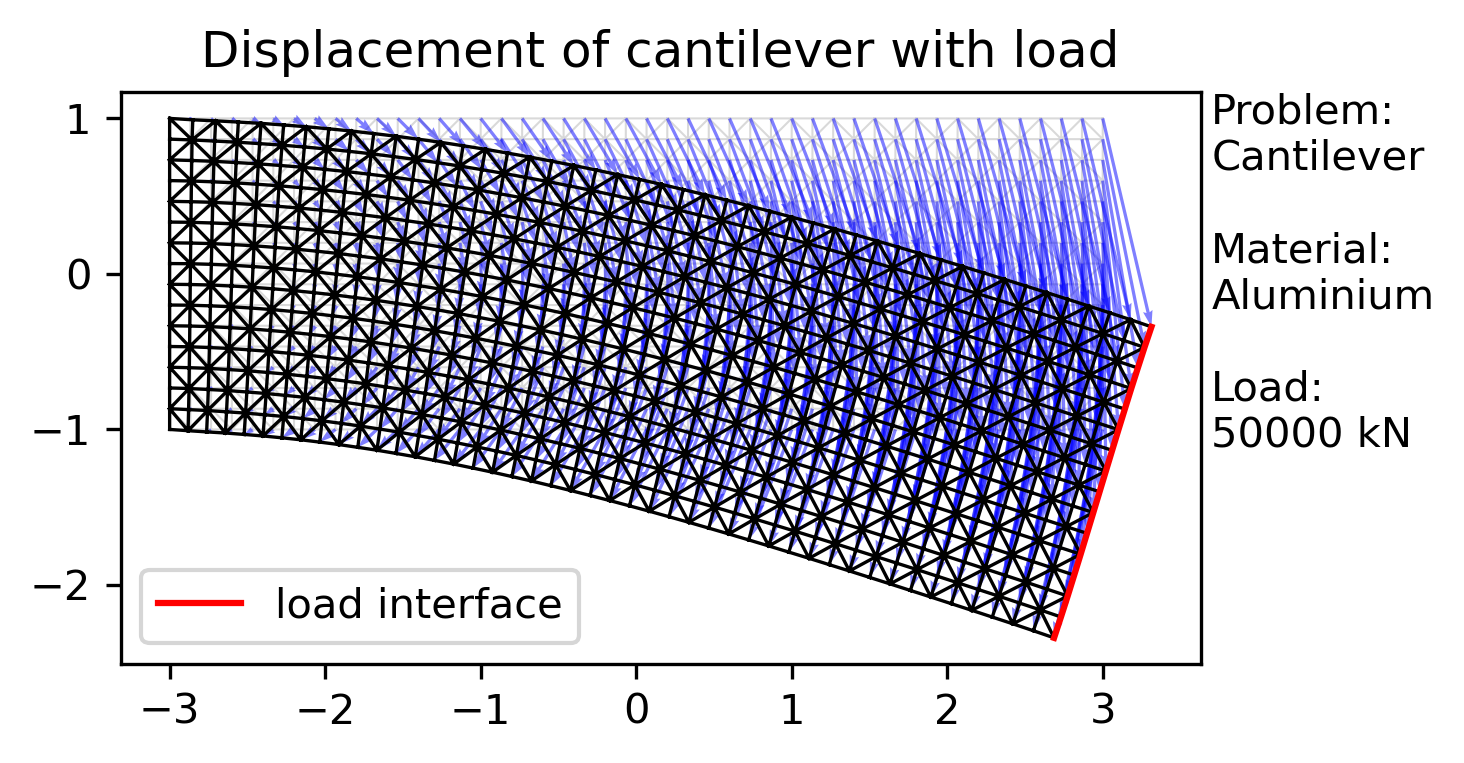
\includegraphics[width = 0.4\textwidth]{exp1_0.png}
  \caption{Deformation of the aluminium beam due to a 50.000 kN traction force.\label{fig:w5exp1_0}}
\end{figure}
\begin{figure}[H]
  \centering
  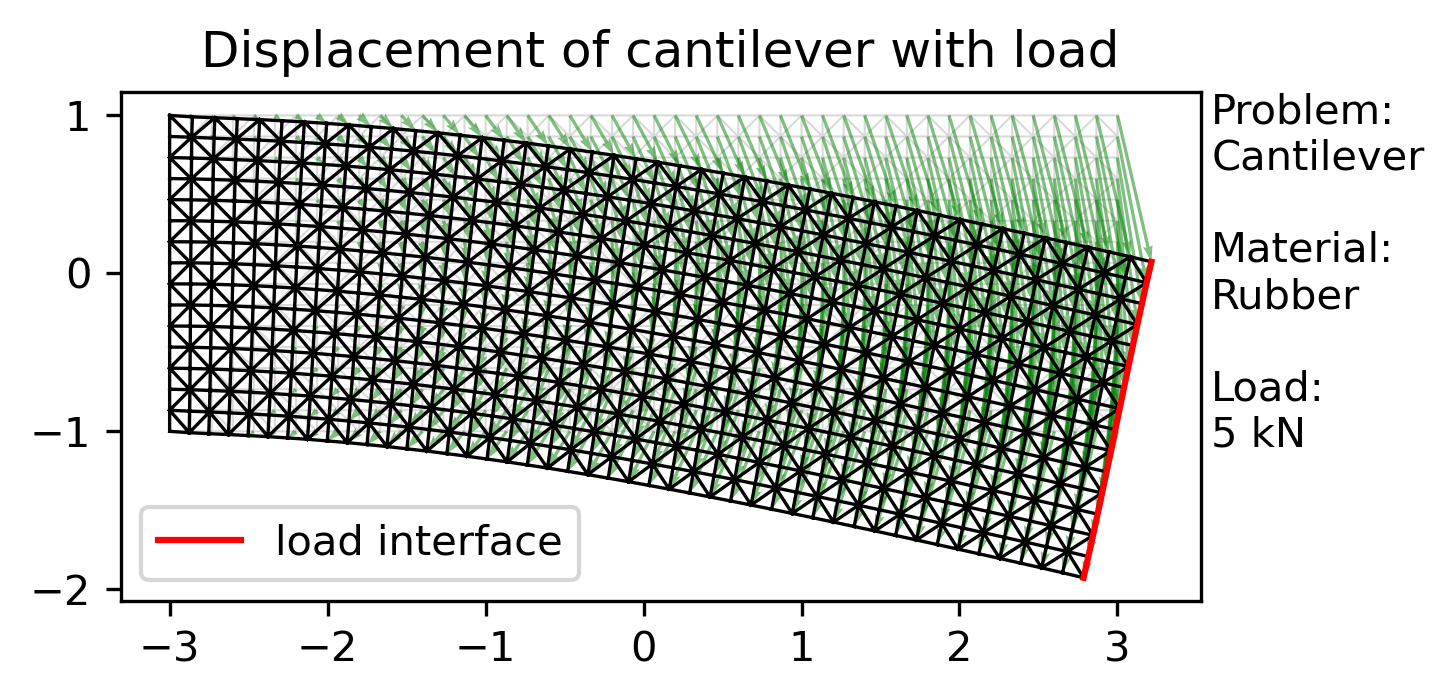
\includegraphics[width = 0.4\textwidth]{exp1_1.png}
  \caption{Deformation of the rubber beam due to a 5 kN traction force.\label{fig:w5exp1_1}}
\end{figure}
%
\vfill
\subsection{Experiment 2: A square block settling under gravity}
In this experiment we try to examine what happens when two square blocks of aluminium and rubber are fixed to a surface and left to settle under gravity. We apply a a gravitational force of $\boldsymbol F_\mathrm{G}  = \rho \boldsymbol g$ to every point on the mesh, and fix the bottom edge, so that $\boldsymbol u(\boldsymbol x_\mathrm{bottom} ) = \boldsymbol 0$. We then calculate the solution for the two blocks. First of all we again expect the rubber to deform more than the aluminium one, but furthermore we expect to see more compression in the bottom of the block as more material is resting on top of it. We also expect the deformation to be symmetric around the middle vertical. In figures \ref{fig:w5exp2_0} and \ref{fig:w5exp2_1} we see that indeed the aluminium block is basically indifferent, while the rubber block is heavliy deformed. Furthermore, the rubber block is more deformed in the bottom than in the top, which is what we expected although there are some problems that needs to be adressed. Our boundary conditions are only applied to the actual bottom points of the mesh, which leads to the "falling over the edge" effect in the final solution. Also the deformation is not symmetrical and seems to favor the left side, and however much we tried we couldn't get rid of this effect. This is probably due to some numerical error, or some mistake in our implementation of the boundary conditions.
%
\graphicspath{{Images/Week5/exp2/}}
\begin{figure}[H]
  \centering
  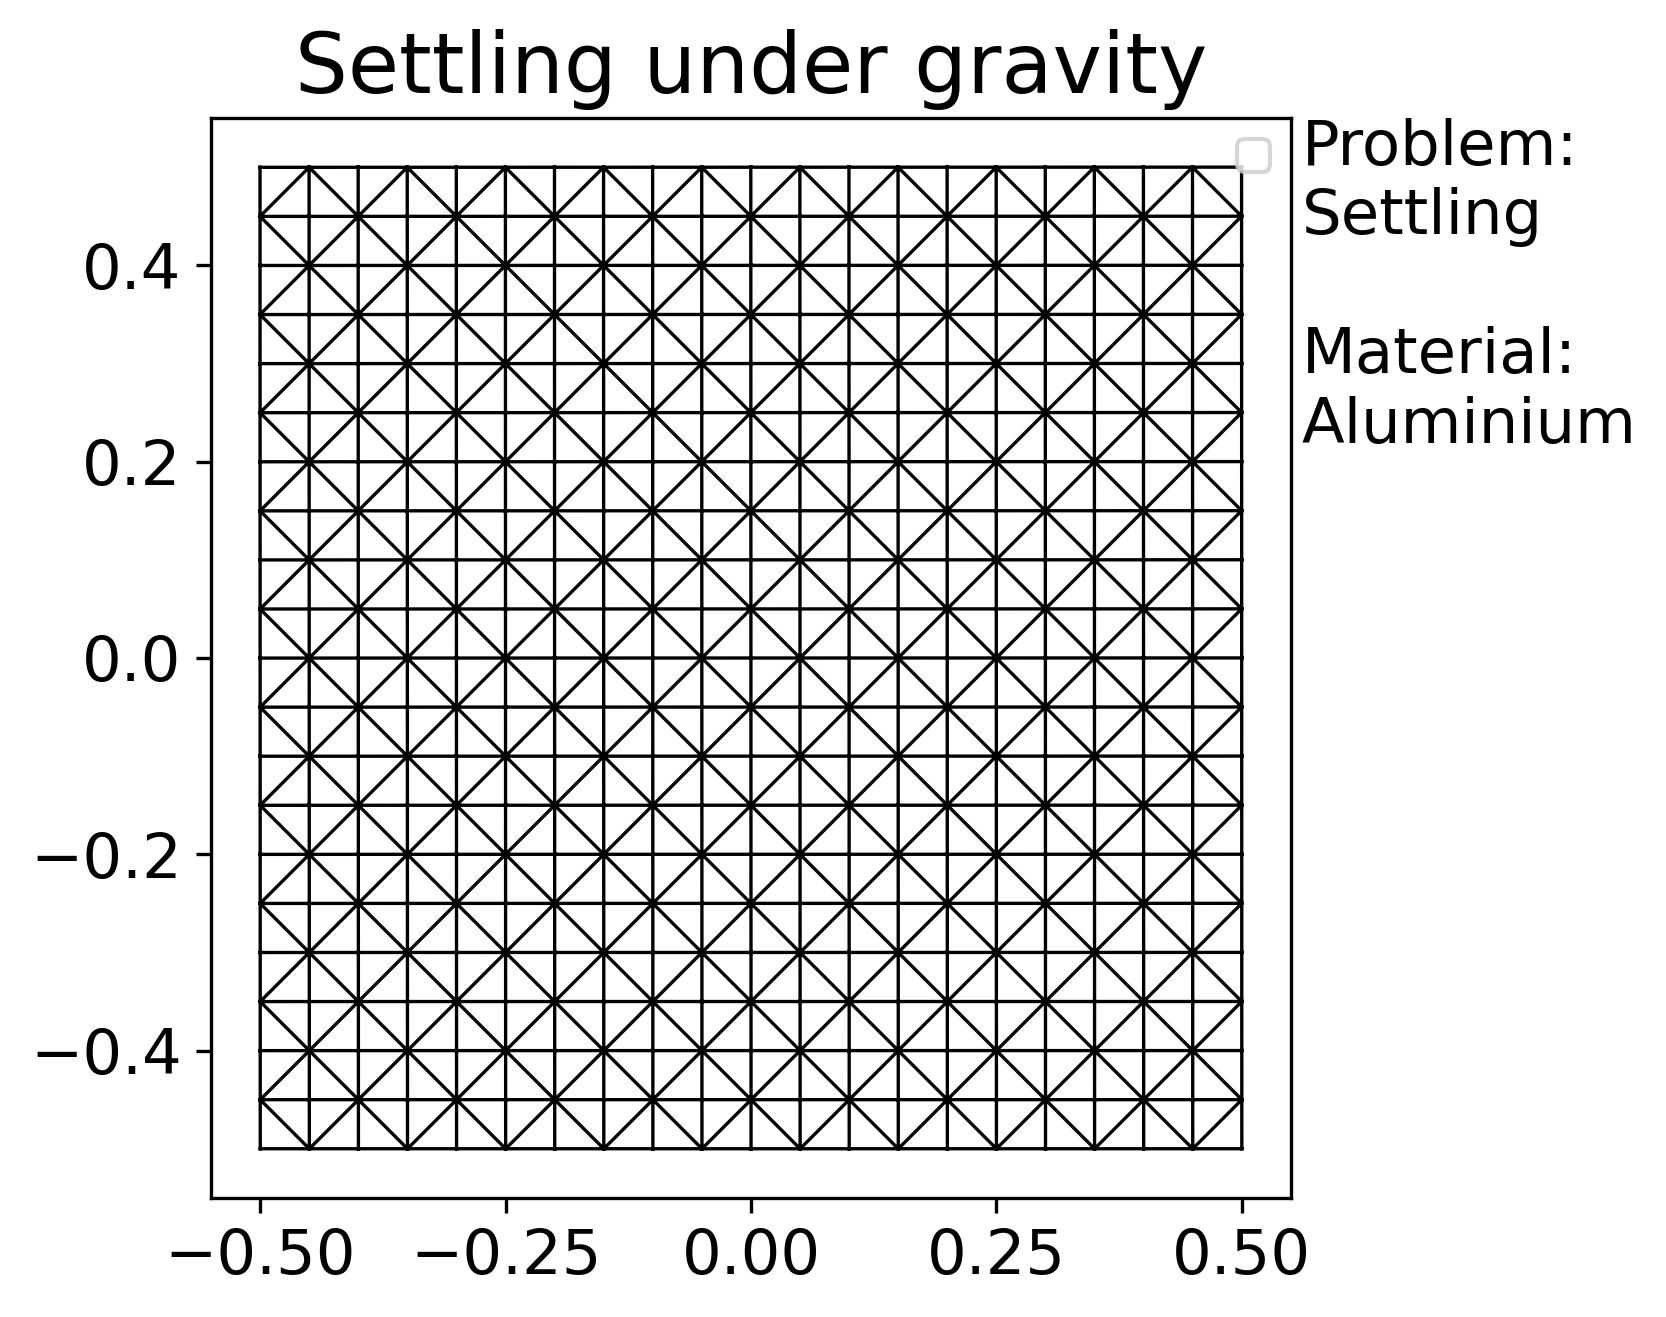
\includegraphics[width = 0.3\textwidth]{exp2_0.png}
  \caption{Deformation of the aluminium block due to its own gravity.\label{fig:w5exp2_0}}
\end{figure}
\begin{figure}[H]
  \centering
  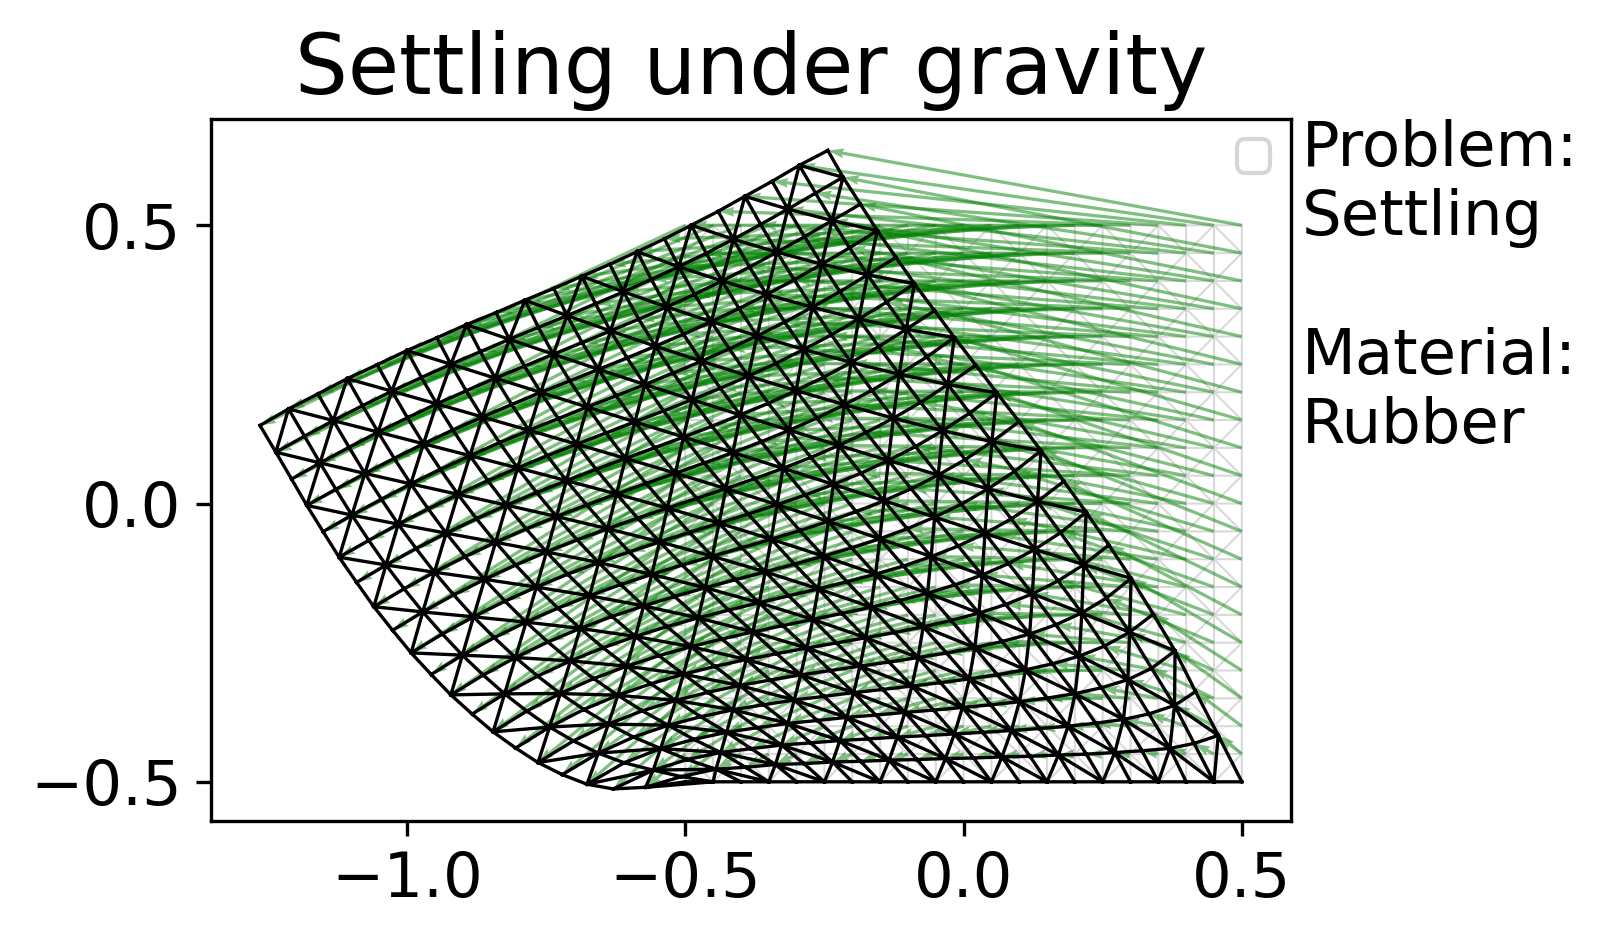
\includegraphics[width = 0.4\textwidth]{exp2_1.png}
  \caption{Deformation of the rubber block due to its own gravity.\label{fig:w5exp2_1}}
\end{figure}


\subsection{Experiment 3: A bridge with a load on top}
In this experiment we want to see how a bridge of aluminium and iron behaves when a load is applied to the top of it. We apply three different loads of 1.000 kN, 5.000 kN and 10.000 kN to the top of the bridges, and fix the left and right edges, so that $\boldsymbol u(\boldsymbol x_\mathrm{left} ) = \boldsymbol u(\boldsymbol x_\mathrm{right} ) = \boldsymbol 0$. Additionally we apply the force of gravity as in the previous experiment.

The elastic parameters of iron are
%
\begin{align}
  E_\mathrm{Fe}   & = 211 \ \mathrm{GPa},     \notag \\
  \nu_\mathrm{Fe} & = 0.29,                    \notag \\
  \rho_\mathrm{Fe} & = 7850 \ \mathrm{kg/m^3}, \notag
\end{align}
%
First of all, we expect the deformation of both bridges to be more pronounced in the middle, and taper off to the sides. We also expect it to be symmetrical around the middle vertical. Additionally we expect the deformation to be of larger magnitude for larger loads. In figures \ref{fig:w5exp3_0}, \ref{fig:w5exp3_1}, \ref{fig:w5exp3_2}, \ref{fig:w5exp3_3}, \ref{fig:w5exp3_4} and \ref{fig:w5exp3_5} we see that the aluminium bridges are more deformed than the iron, and that the deformation is more pronounced in the middle of the bridge. Furthermore we see here that the deformation is symmetrical around the middle vertical, which is in contrast to the previous experiment. This is probably due to the fact that the boundary conditions are applied to both vertical edges of the mesh, and not only to the bottom points. We also see that the deformation is more pronounced for larger loads, which is what we expected.

\graphicspath{{Images/Week5/exp3/}}
\begin{figure}[H]
  \centering
  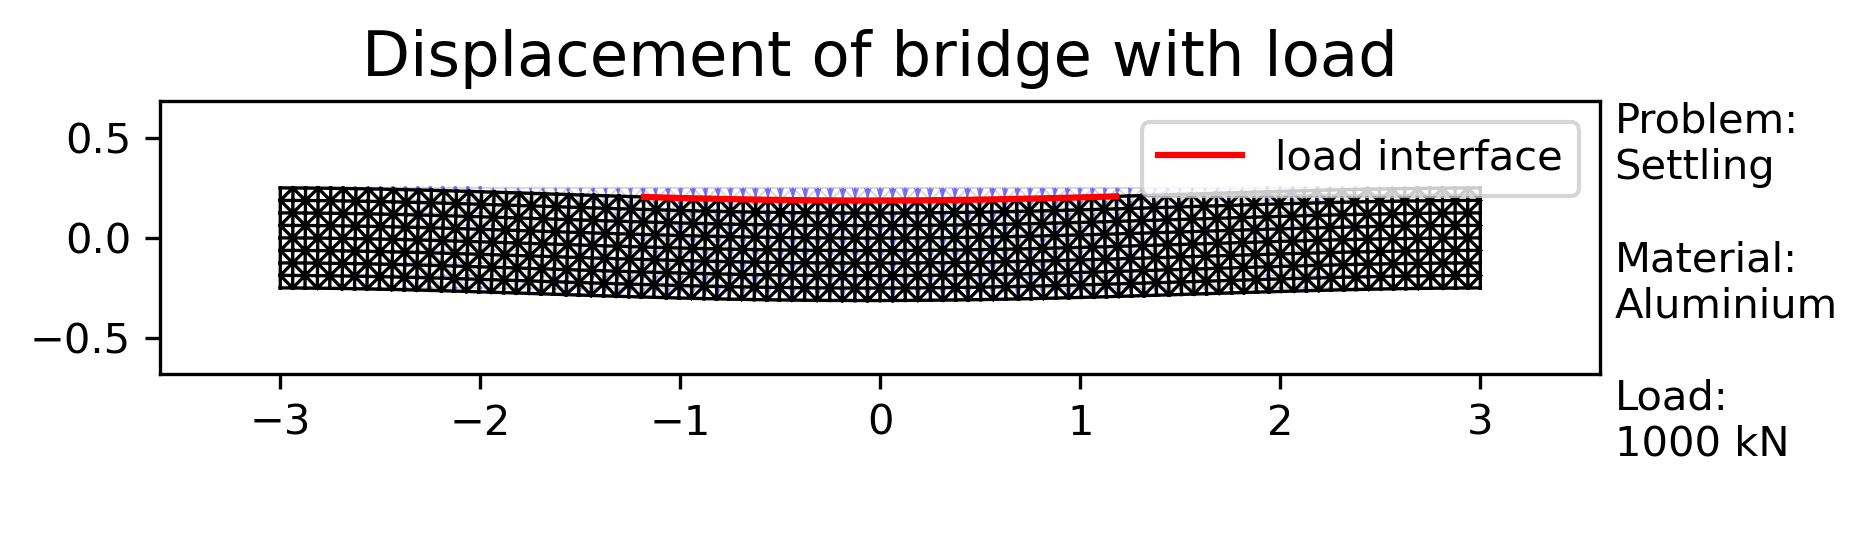
\includegraphics[width = 0.5\textwidth]{exp3_00.png}
  \caption{Deformation of a aluminium due to 1.000 kN load on top.\label{fig:w5exp3_0}}
\end{figure}
\begin{figure}[H]
  \centering
  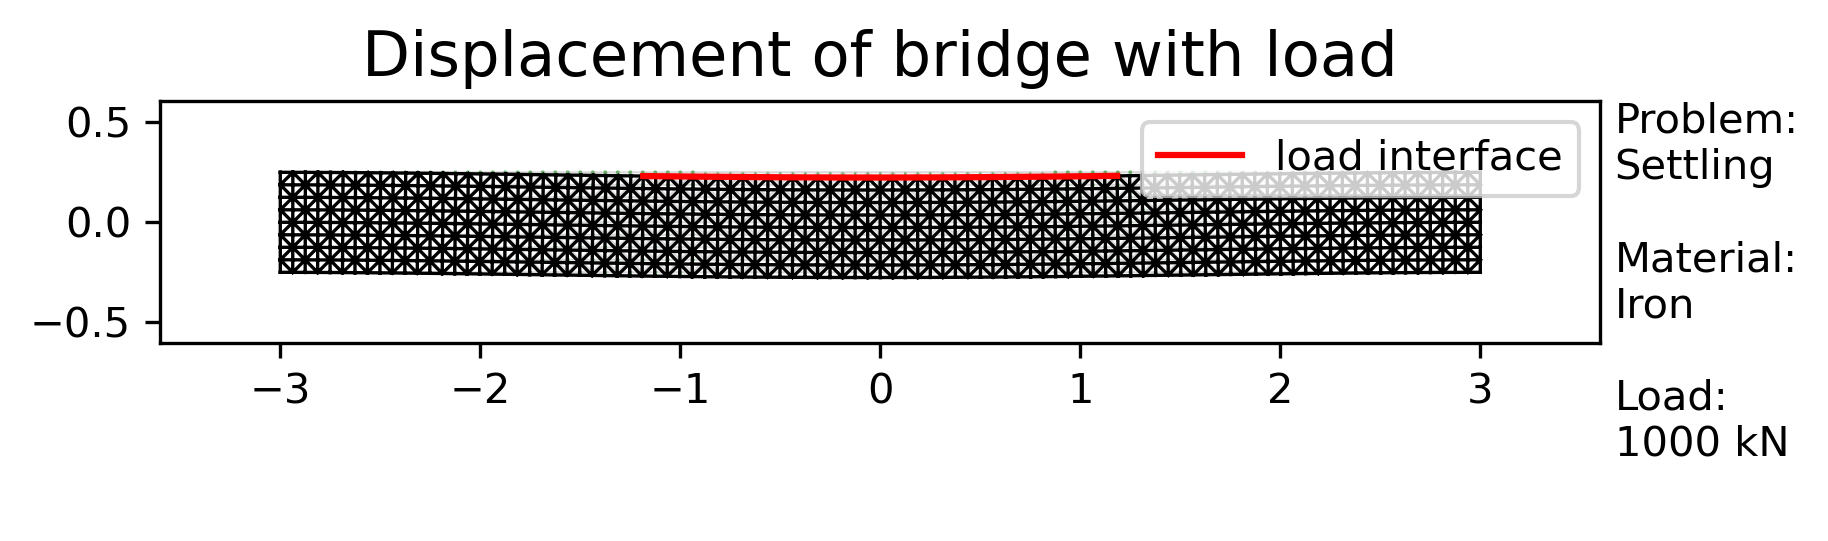
\includegraphics[width = 0.5\textwidth]{exp3_01.png}
  \caption{Deformation of a iron due to 1.000 kN load on top.\label{fig:w5exp3_1}}
\end{figure}
\newpage
\begin{figure}[H]
  \centering
  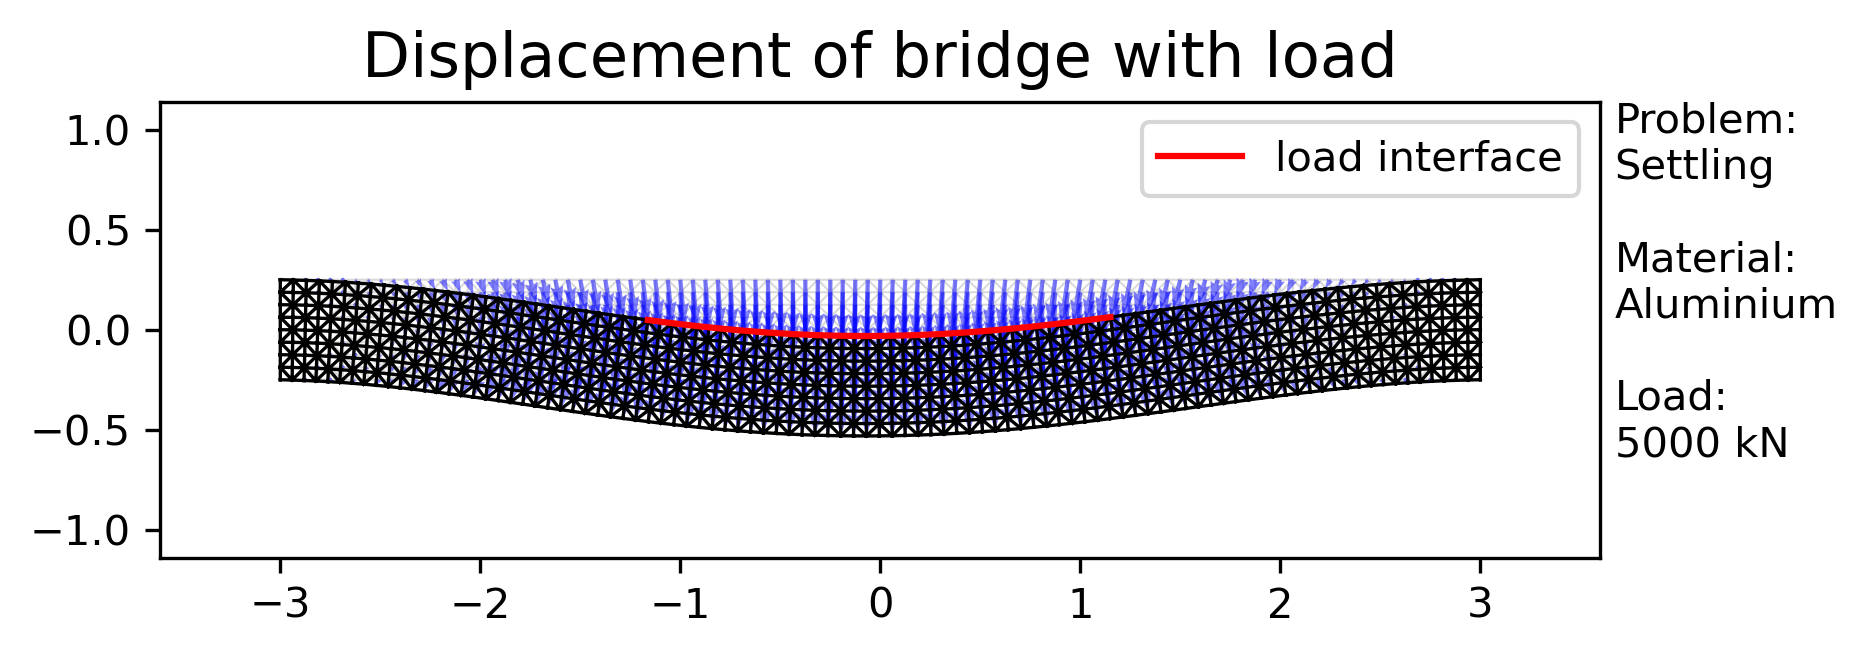
\includegraphics[width = 0.5\textwidth]{exp3_10.png}
  \caption{Deformation of a aluminium due to 5.000 kN load on top.\label{fig:w5exp3_2}}
\end{figure}
\begin{figure}[H]
  \centering
  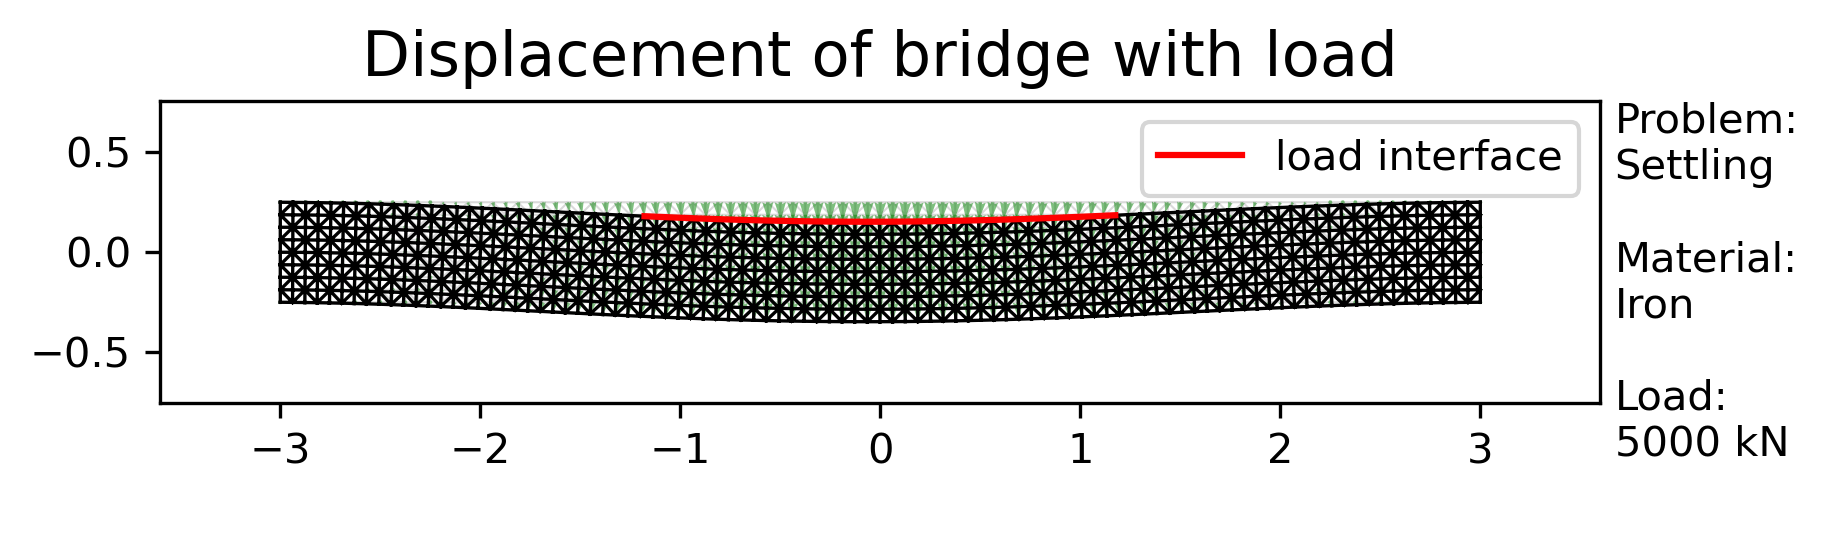
\includegraphics[width = 0.5\textwidth]{exp3_11.png}
  \caption{Deformation of a iron due to 5.000 kN load on top.\label{fig:w5exp3_3}}
\end{figure}
\begin{figure}[H]
  \centering
  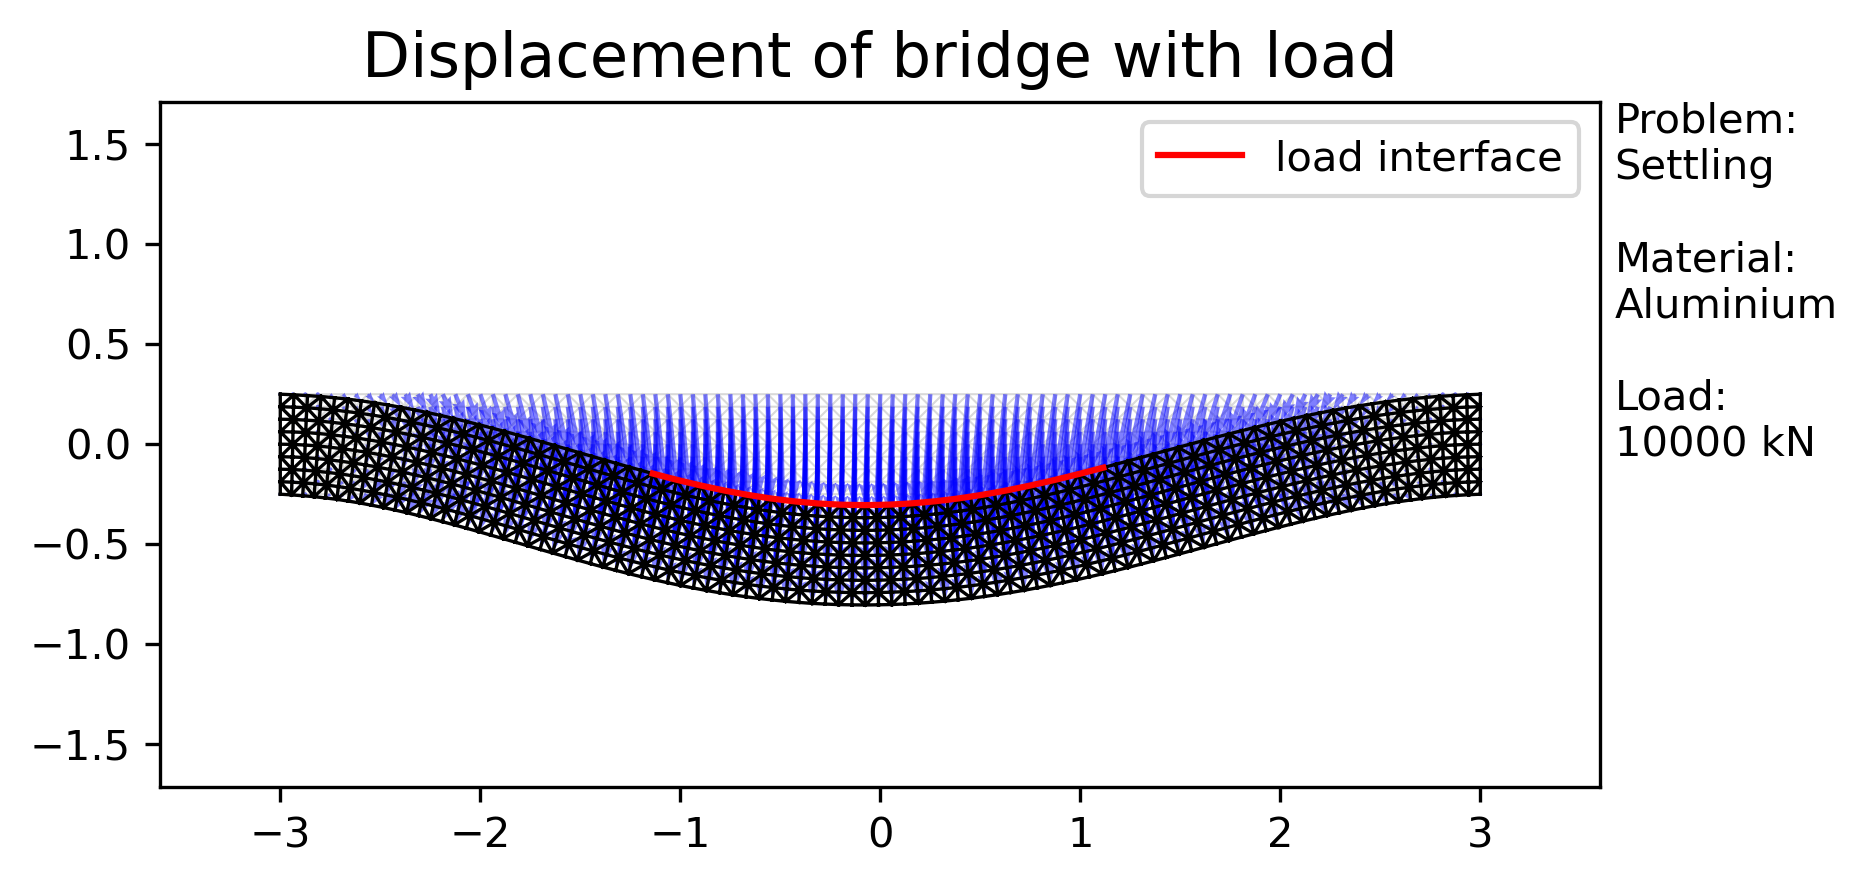
\includegraphics[width = 0.5\textwidth]{exp3_20.png}
  \caption{Deformation of a aluminium due to 10.000 kN load on top.\label{fig:w5exp3_4}}
\end{figure}
\begin{figure}[H]
  \centering
  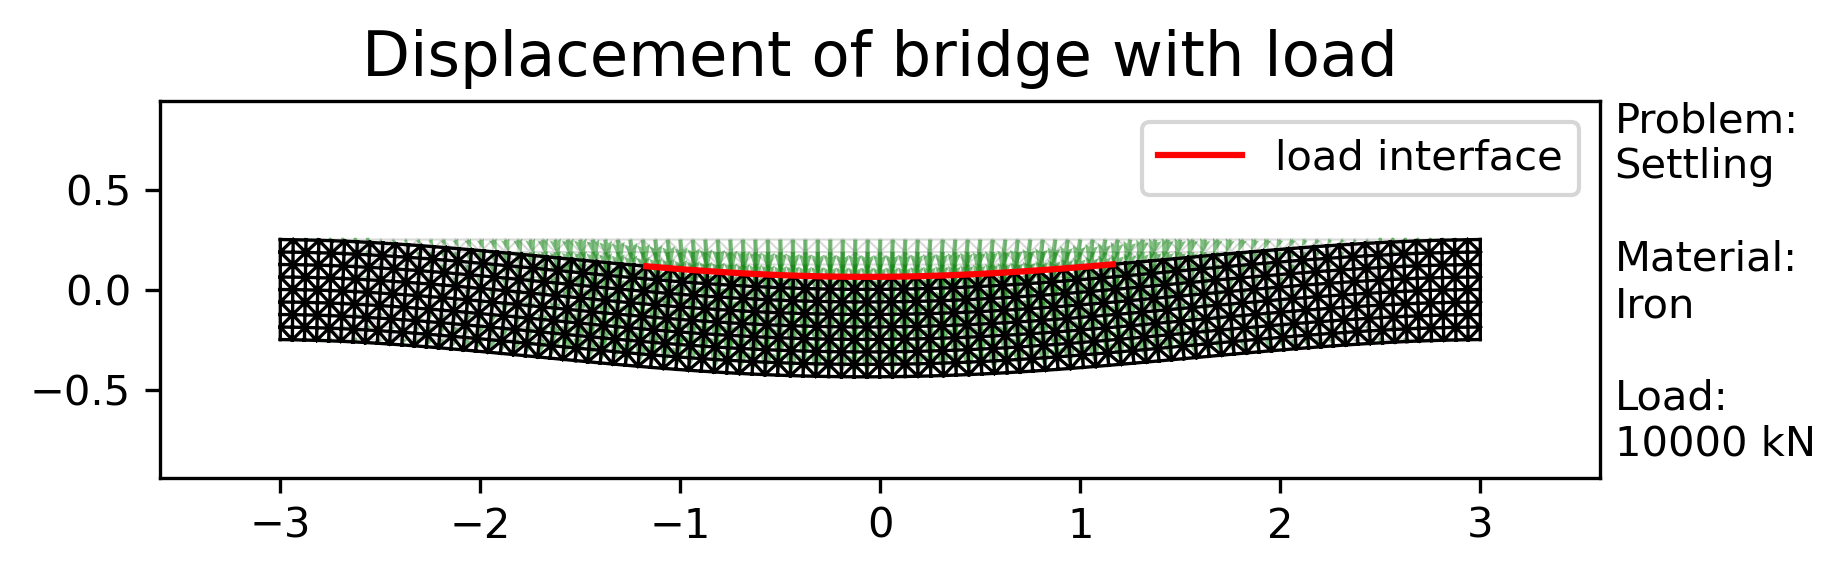
\includegraphics[width = 0.5\textwidth]{exp3_21.png}
  \caption{Deformation of a iron due to 10.000 kN load on top.\label{fig:w5exp3_5}}
\end{figure}

\end{document}
\endinput
